%%%%%%%%%%
% [TODO] %
%%%%%%%%%%
% [ ] Mini-intro
% [ ] PhonMatch
%%% [ ] k-epenth
%%% [X] wpd
% [ ] Mini-discussion

%%%%%%%%%%%%%%%%%%%%%%
% Chapter mini-intro %
%%%%%%%%%%%%%%%%%%%%%%
\section{Introduction}
%%% Short BG
%\subsection{ASR tools as models of perception}
% Test acoustic model (null)
% Compare with more informative LMs
% Qualitative testing on best LM
% Investigate phonetic match - wpd/phonological alt 


%%% Research question + alternatives


%%% Plan


%%%%%%%%%%%%%%%%%%%
% General methods % %
%%%%%%%%%%%%%%%%%%%

\section{Anatomy of our HMM-based speech recogniser}
For the experiments described in this chapter we used Hidden Markov Model (HMM)-based speech recognisers as models of human perception. 
Speech audio waveforms are transformed into a sequence of \textbf{acoustic vectors} $X_{1:T} = x_{1}, ..., x_{T}$ through the first step, called feature extraction. In the decoding phase that follows, the trained ASR system attempts to find the sequence of words $w_{1:L} = w_{1}, ..., w_{L}$ which is most likely to have produced the sequence of acoustic feature vectors $X$.
Mathematically, this equates to solving the following equation:

\begin{equation}
  \widehat{w} = \underset{w}{arg\,max} \left \{  P(w|X)\right \}
  \label{eq_hmm_dec_post}
\end{equation}

Put into Bayesian terms, this represents computing the posterior probability $P(w|X)$ of all combinations of words, given the acoustics, and retrieving the index of the most probable one: the decoder selects the sequence of words $w$ with highest posterior probability given the acoustic evidence $X$. However, due to the fact that there is an infinite number of possible combinations of words, it may be difficult to evaluate all possible combinations in order to find the most probable one. As such, following Bayes's theorem, equation \ref{eq_hmm_dec_post} can be rearranged as:

\begin{equation}
  \widehat{w} = \underset{w}{arg\,max} \left \{  P(X|w)P(w)\right \}\footnote{In practice $P(X|w)P(w)$ is often computed in the log space as $\alpha ~log P(X|w) + log P(w)$, where $\alpha$ is a scaling factor called acoustic scale (set to $0.1$ in our models)}
  \label{eq_hmm_dec_post}
\end{equation}
The likelihood $P(X|w)$, given by the \textbf{acoustic model}, is the probability of the acoustics given the sequence of words. The prior $P(w)$, given by the \textbf{language model}, corresponds to the probability of the word sequence, and can be derived from frequency counts. These probabilities can be extracted by training our ASR system using annotated speech corpora.

Nowadays, in the field of ASR, Neural Network (NN)-based speech recognisers are the state-of-the-art. In spite of better performance of NN-based ASR systems, we decided to use HMM-based recognisers, which are better understood than NNs while still offering good speech recognition performance. Indeed, before the decoding step, these models offer a clear separation between the acoustic model (AM; i.e., mapping between phoneme categories and acoustics) and the language model (LM; i.e., frequencies of word/phoneme sequences). This allowed us to test ASR systems with different LMs while keeping the AM constant, as well as adapting LMs to mimic the experimental paradigms used when testing human participants. Importantly, unlike NNs which are often qualified as ``black boxes'', we are able to better understand and analyse how the ASR system processes acoustic input. 
We will now present the necessary components for building an HMM-based ASR system, namely the speech corpora used to train and test the system and its featural representation, as well as the decoder itself, composed of an acoustic model, a lexicon, and a language model. The interaction of these elements is depicted in Figure \ref{fig:hmm_architecture}. In the following subsections we will present the components in more detail. 

\begin{figure}[htb]
\centering
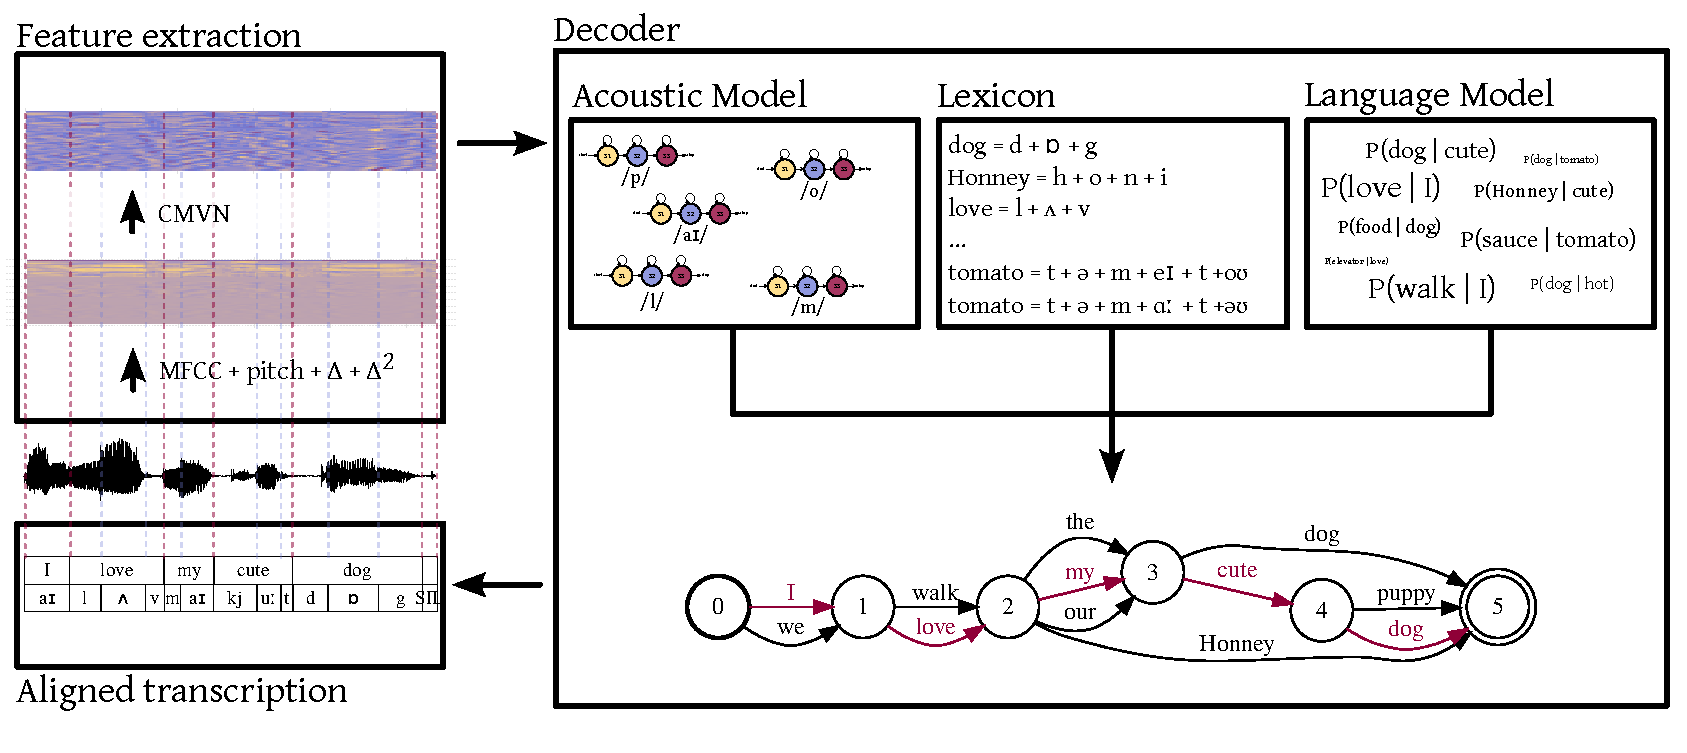
\includegraphics[width=1\linewidth]{chapter03/hmm_all_version2.pdf}
\caption{\textit{Architecture of our ASR system, including its input (acoustic features) and output (transcription).}}
\label{fig:hmm_architecture}
\end{figure}

\subsection{Corpora}

In order to train and test our ASR system, we required transcribed speech corpora. These corpora consisted of speech recordings which have been annotated; for each utterance, we have a more or less detailed transcription of what was said.
While the ideal annotation is one for which phoneticians have provided phoneme categories (or even phones), as well as their boundaries, often we might only have access to by-utterance annotations where we are only provided with a sequence of words/phonemes for each utterance. In these cases, we rely on forced alignment to automatically find phoneme boundaries.

In the following sections we have trained ASR systems with different ``native'' languages, namely Japanese (JP) and Korean (KR). These languages were of particular interest because of their relatively restrictive phonotactics with regards to consonant clusters, as well as the availability of corpora of spontaneous speech, which we will now present. We also trained an American English (EN) corpus in order to evaluate our model's performance with respect to state-of-the-art systems. 

\paragraph{Corpus of Spontaneous Japanese (CSJ)}
As the name suggests, the CSJ \cite{maekawa2003} contains recordings of spontaneous Standard Japanese. The corpus is composed of two subparts: (1) academic presentation speech (APS), which consists of live recordings of academic presentations, and (2) simulated public speech (SPS), where speakers presented everyday topics in front of a small audience. For our models we only kept SPS, which is more representative of everyday conversations at the level of the lexicon, and has a more balanced population than the young, male-dominated APS.
Recordings were manually transcribed by native speakers of Japanese using Japanese syllabaries, which meant that the phonetic transcriptions only included phonotactically legal phoneme sequences, even in cases where the actual acoustics might have been closer to illegal sequences. Phoneme boundaries were manually adjusted; however, this alignment was not used when training our models, as it was overwritten by forced alignment due to technical constraints.
Our subset of the corpus contained $400,547$ utterances produced by $594$ speakers\footnote{For the CSJ and KCSS, we used utterances from the same speakers for the validation and test sets, but their data was not seen during model training. For the WSJ, data from all speakers was used in the 3 corpus subsets, due to a planned comparison to another corpus not described here. Since the speakers that we used in our experiments are not from any of the corpora, this is not an issue. However, it needs to be kept in mind that error rates (\%WER and \%PER) for KCSS, CSJ, and WSJ are only comparable within corpus.} ($331$ female, $263$ male), with an average of $674.3$ utterances per speaker. The division of the corpus across training, validation, and test set are shown in Table \ref{tab:hmm_csj}.

\begin{table}[htb]
\centering
\caption{Datasets used for training and evaluating the Japanese ASR system with the CSJ.}
\label{tab:hmm_csj}
\vspace{0.25cm}
\begin{tabular}{rrrrrr}
  \toprule
      & Proportion &\# Utterances & Duration (hh:mm:ss) & \# Speakers &  \\ \midrule
  train & $80\%$ &  $322,208$            & 152:26:33     &   475          &  \\
  valid & $5\%$ &  $19,566$         &  9:12:03    &   119          &  \\
  test  & $15\%$ &  $58,773$        &  27:19:14    &  119           & \\ \bottomrule
\end{tabular}
\end{table}

\paragraph{Korean Corpus of Spontaneous Speech (KCSS)}

The KCSS \cite{yun2015} consists of recordings of spontaneous Seoul Korean. Forty speakers aged $10$ to $49$ ($5$ female speakers and $5$ male speakers per decade) were recorded in a quiet room, for approximately 1 hour each. Speech was ellicited through questions related to the speakers' personal opinions, habits, acquaintances, etc.      
Recordings were manually transcribed by native speakers of Korean. We used phonetic transcriptions faithful to actual pronunciations which, for instance, include phonetic reduction (akin to \textit{yesterday} being transcribed as \textipa{/jESeI/} instead of the canonical \textipa{/jEst\textrhookschwa deI/}). The transcription process involved the use of the main writing system of Korean (i.e., hangul) as well as a romanization, meaning that there is a possibility that acoustic sequences closer to phonotactically illegal sequences might have been transcribed as phonotactically legal counterparts.   
Transcriptions include manually adjusted phoneme boundaries, as well as word syllabification; however this alignment was not used when training our models, as it was overwritten by forced alignment due to technical constraints.
%{\color{red}[NOTE]: \%WER for mono-pitchT-1000 is 81.1\% with forced alignment and ... 99.3\% when ``using the manual alignment''!!!! For this latter, many words as transcribed as ``$<$unk$>$'', so something is very wrong. Maybe at the level of the ali.*.gz files?}
The corpus contains $57,504$ utterances produced by $40$ speakers (as explained above), with an average of $1,437.6$ utterances per speaker. The division of the corpus across training, validation, and test sets is shown in Table \ref{tab:hmm_kcss}.

\begin{table}[htb]
\centering
\caption{Datasets used for training and evaluating the Korean ASR system with the KCSS.}
\label{tab:hmm_kcss}
\vspace{0.25cm}
\begin{tabular}{rrrrrr}
  \toprule
      & Proportion & \# Utterances & Duration (hh:mm:ss) & \# Speakers &  \\ \midrule
  train & $80\%$ &  $46,208$ &   18:58:15   &   $32$    &  \\
  valid & $5\%$ &  $2,824$ &  1:16:39  &  $8$  &  \\
  test  & $15\%$ &  $8,472$ & 3:54:15   & $8$    & \\ \bottomrule
\end{tabular}
\end{table}

\paragraph{Wall Street Journal - Read (WSJ)}
The WSJ \cite{paul1992} is a corpus of both read and spontaneous American English.
For our work, we only kept the read subset of the corpus, which consisted of {\color{red}professionally trained journalists} recorded while reading news articles. Contrary to the CSJ and KCSS, the recordings were not phonetically transcribed. However, we had access to the news articles themselves, as well as to a dictionary which mapped the standard phonetic pronunciation of words in American English to the words in the articles.
In total, $338$ speakers {\color{red}($X$ female, $Y$ male)} uttered $71,037$ utterances, with an average of $210.2$ utterances per speaker. The division of the corpus across training, validation, and test sets is shown in Table \ref{tab:hmm_wsj}. 

\begin{table}[htb]
\centering
\caption{Datasets used for training and evaluating the American English ASR system with the WSJ corpus.}
\label{tab:hmm_wsj}
\vspace{0.25cm}
\begin{tabular}{rrrrrr}
  \toprule
      & Proportion & \# Utterances & Duration (hh:mm:ss) & \# Speakers &  \\ \midrule
  train & $80\%$ &  $56,872$ &   115:18:46   &   $338$    &  \\
  valid & $5\%$ &  $3,661$ &  7:24:22  &  $338$  &  \\
  test  & $15\%$ &  $10,504$ & 21:12:19  & $338$    & \\ \bottomrule
\end{tabular}
\end{table}
      
\subsection{Features}
In order for our ASR systems to be able to use speech as input, it is necessary to perform signal analysis. This procedure transforms the continuous raw speech waveform into sequential speech features. This latter form ensures a more more informative representation of speech, with modifications that enhance phonemic contrasts and better approximate how speech is processed by the human cochlea. In this work we used Mel-frequency cepstrum coefficients (MFCC), traditionally used for HMM-based ASR systems.

Speech is recorded with a microphone; the continuous audio signal is digitalized at a sampling rate of 16kHz.
The audio is then segmented into frames of 25 ms, with a shift of 10 ms between the beginning of each frame. By using frames, we make the assumption that the signal is stationary within the 25 ms window, and we apply the following proccessing steps to each frame, using Kaldi \cite{povey2011}:

\begin{enumerate}
\item Pre-processing: The data is extracted and pre-processed (dithering, pre-emphasis, and DC offset removal).
\item Windowing: The data in the 25 ms frame is multiplied by a tapered window (Hamming window), to avoid discontinuities at the edges of the segment.
\item Spectral analysis: By applying a Fast Fourier Transform (FFT), we find out how much energy there is at each frequency band for this frame.
\item Nonlinear frequency scaling: In order to compensate for the fact that human hearing is less sensitive to higher frequencies, frequencies are mapped onto a Mel scale, which is linear until approximately 1000 Hz and logarithmic afterwards. This is done by applying a mel-filter bank with 23 bins, which are equally spaced in the mel-frequency domain. Each filter summarises the amount of energy in a section of the range of frequencies. 
\item Cepstral analysis: The log of the energy in each bin is computed, from which we take the cosine transform. We keep 13 MFCCs, including $c_{0}$, the zeroth coefficient which represents the average of the log-frequency of the bins \cite{gales2008}.
  \item Cepstral liftering: Coefficients are scaled, ensuring that they have a reasonable range.
\end{enumerate}

We therefore obtain 13 MFCCs that summarise the information at each frame of audio. To these coefficients, we add 3 coefficients carrying information about pitch: normalized-pitch, delta-pitch, voicing-feature\footnote{Information about pitch was added because of its contrastive relevance in Japanese at the lexical level (i.e., pitch accent) and in Korean at the phonemic level (e.g., tonogenesis in the three-way contrasts of plosives). In practice, adding pitch features resulted in a slight improvement of model performance in Japanese (from $41.3\%$ WER to $39.6\%$; acoustic model with 6000 Gaussians).}.
To these 16 static features we add their respective dynamic features ($\Delta$ and $\Delta^2$) that describe the evolution of the coefficient values over time. 
Coefficient values are then standardised using Cepstral Mean Variance Normalisation (CMVN); for each speaker the distribution of each coefficient's values has a mean value of zero and a variance of one. 

\subsection{Acoustic model}

Now that we have extracted the acoustic features for the labelled utterances in our corpus, we are able to train the acoustic model (AM). Recall that the AM gives the likelihood $P(X|w)$, which corresponds to the probability of the acoustics given the sequence of words $w$.
In order to simplify things, let's not view an utterance as a sequence of words which are sequences of phonemes themselves, but directly as a sequence of phonemes. Then, we consider the probability of the acoustics $X$ given the sequence of phonemes $W$.
The acoustics corresponding to a given phoneme change during the duration of the phoneme; as such, phones are not static objects but they should be described as having acoustic trajectories. By using Hidden Markov Models (HMM), we can approximate these trajectories as sequences of static states. A priori, the more states, the better the approximation to the real data. However, empirically it has been assessed that having three states is a good compromise for ASR systems. Following this, we chose to model phonemes as three-state HMMs, where the states correspond, respectively, to the beginning, middle, and end portions of the phoneme. This is particularly relevant for phonemes that can be viewed as sequences of discrete articulatory events with distinct acoustic signatures, such as plosives (e.g., \textipa{/p/}) which are often described as an airway closure, followed by a period of occlusion and a possibly audible release. Additionally, the separation into three states allows to account for the fact that the acoustics of the beginning and end of a phoneme may be differently affected by neighbouring phonemes (i.e., coarticulation) in comparison to the medial part. 

As their name suggests, HMMs follow a Markovian process; the value of a state only depends on the value of the previous state. The transitions between states are defined by transition probabilities not only between adjacent states, but also within a state itself (i.e., self-loops). These transition probabilities are defined during AM training, based on the transitions between frames in the training corpus. While the duration of phonemes cannot be explicitly learned by the acoustic model, they are implicitly reflected by the transition probabilities in the self-loops: for a given state, the higher the self-loop probability, the longer the model will ``remain'' at said state and the longer the sequence of acoustic vectors assigned to the corresponding phoneme. A simplified illustration of a phoneme HMM is shown in Figure \ref{fig:hmm_3state}.

\begin{figure}[htb]
\centering
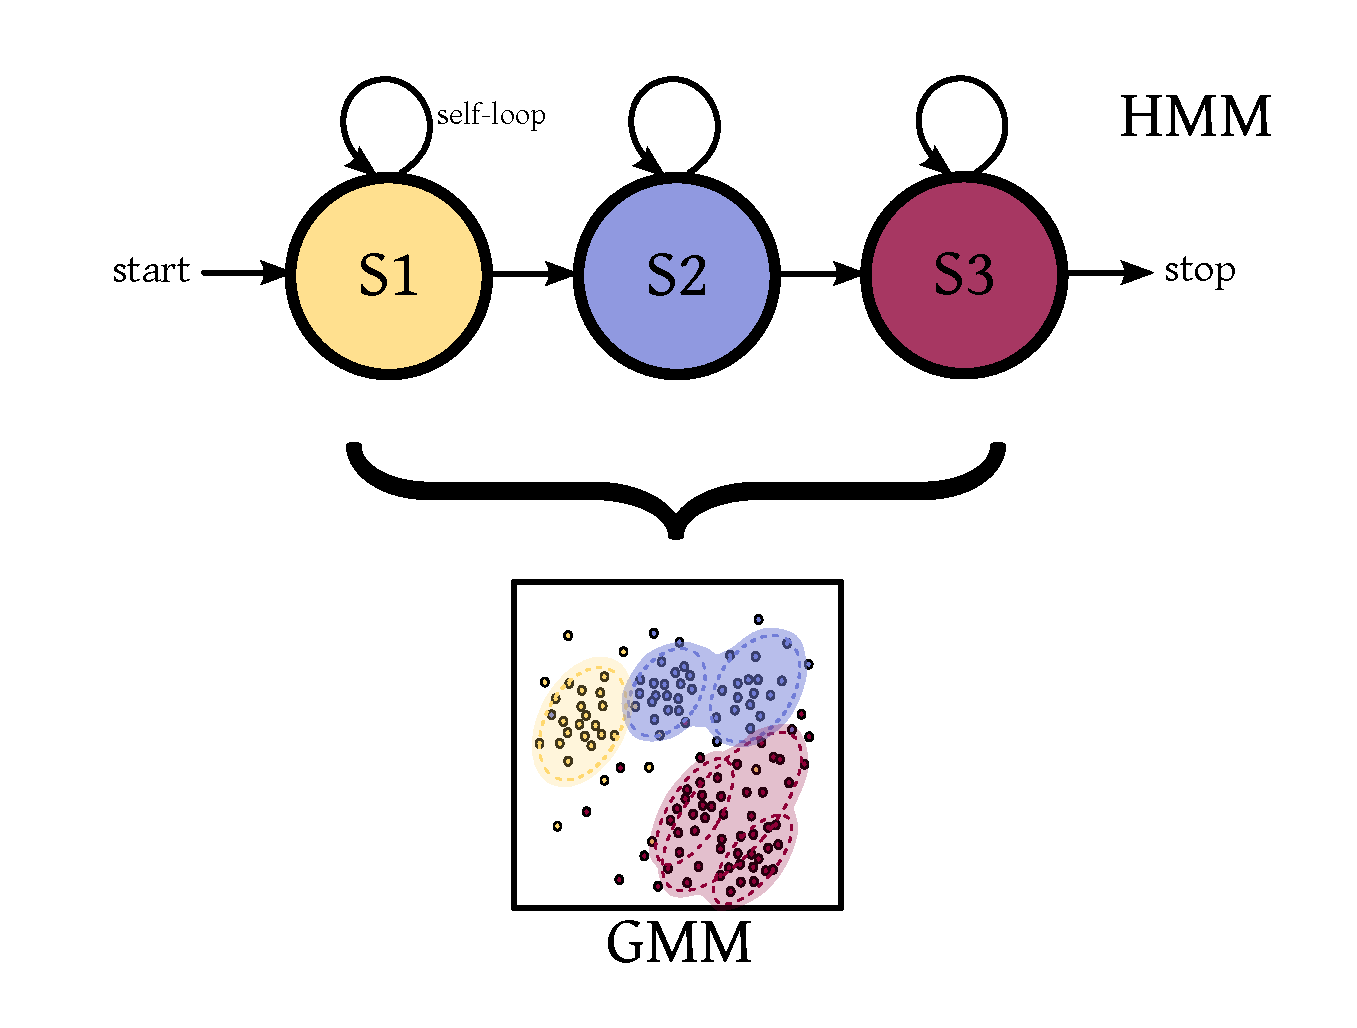
\includegraphics[width=0.6\linewidth]{chapter03/hmm_3state.pdf}
\caption{\textit{Left-to-right 3-state phoneme HMM with simplified 2-dimensional GMM (one per state). Start and stop states connect the phoneme with the previous and next phoneme, respectively.}}
\label{fig:hmm_3state}
\end{figure}

In sum, each phoneme is modelled by a left-to-right 3-state HMM. But what exactly is a state? Our acoustic models are HMM-GMMs, where GMM stands for Gaussian Mixture Models. For each phoneme our 48-dimensional feature vectors define a 48-dimensional space where GMM for the three states are embedded. During training, the acoustic model will have placed individual acoustic frames on this space, based on the values of their feature vector. In other words, acoustic frames from each phoneme portion will occupy a certain part of this space. For each state, we can parametrically define the space covered using mixtures of Gaussian distributions (the aforementioned GMMs). Indeed, GMMs are universal approximators of densities when given enough components. To do this, the model will have fitted a number of diagonal Gaussian distributions to approximate the distribution of datapoints corresponding to each phoneme state. The number of Gaussians allocated to each phoneme state depends on the total number of Gaussians made available to the model, and the complexity of the distribution of the frames in the space. Once that the GMMs are defined, the AM is able to tell us, for any new frame, the likelihood that the frame originated from each GMM (i.e., phoneme state).  \\     

\subsubsection{Why not triphones?}
If the reader is already familiar with ASR systems, they may expect us to go a step further and no longer treat phonemes as units for the HMMs (i.e., monophone acoustic models) but, instead, use context-dependent triphones. In this latter representation, an independent three-state HMM is built for each phoneme within a phonemic context. With some simplifications, this equates to no longer having an HMM for the phoneme \textipa{/p/}, but having all context-dependent versions of this phoneme as individual HMMs (e.g., the triphone \textipa{/p$_{a\_i}$/}, which is the phone \textipa{/p/} when preceded by \textipa{/a/} and followed by \textipa{/i/}).
Traditionally, triphone-based HMM-based ASR systems perform better than monophone systems. However, these more complex models are inappropriate for our experiments. Recall that we aim to use these speech recognition systems as models of nonnative speech perception, using tasks analogous to paradigms used in psycholinguistic experiments (namely, identification/forced-choice tasks). Importantly, we are focusing on modelling perceptual vowel epenthesis. This situation excludes the use of triphones because, by definition, our ASR systems will have to decode speech that does not follow native phonotactics. Decoding such stimuli implies the existence of triphones corresponding to the input, yet the model will have never encountered such triphones in the training data. While this situation might seem analogous to what listeners may experience, one must consider the fact that the ASR system \textit{will attempt to account for said triphones} during decoding in spite of the lack of data. Importantly, poorly estimated, phony triphones (e.g., \textipa{/h$_{a\_p}$/}, when decoding \textipa{/ahpa/}) will be put up against well-estimated triphones (e.g., \textipa{/h$_{a\_a}$/}) during the forced-choice tasks. The well-estimated triphones might simply be preferred as transcriptions over poorly-estimated ones for this reason alone, irrespective of the actual acoustic match between the stimuli and phoneme models.
In order to increase the performance of monophone models at phonetic labelling tasks such as ours, it is possible to increase the number of total Gaussians available to the model \cite{saraclar2001}. 

\subsection{Lexicon \& language models} \label{hmm_lm}
As shown in Figure \ref{fig:hmm_architecture}, the acoustic model is combined with two other components in order to decode speech: the Lexicon and the Language Model (LM).

The lexicon is, put simply, a pronunciation dictionary. It links the acoustic model (i.e., phoneme-level HMMs) with the language model, which is at the word level. For each word, we indicate in the dictionary the sequence of phonemes that constitute it. It is also possible to account for multiple pronunciations of a word due to dialectal differences (e.g., ``tomato'' pronounced as \textipa{/t@mA:t@U/} or \textipa{/t@meIRoU/}), phonological phenomena (e.g., homorganic assimilation: ``handbag'' \textipa{/h\ae ndb@g/} $\rightarrow$ \textipa{/h\ae mb@g/}), or supresegmental information (e.g., stress contrasts: ``record'' \textipa{/'rekord/} (noun) vs. \textipa{/re'kord/} (verb)).

At the word level, the language model specifies $P(W)$, the probability of occurrence of word sequence $W$. For this we use \textit{n}-grams: we approximate the probability of a sequence
\begin{equation}
P(W) = P(w_{1})P(w_2|w_1)P(w_3 | w_1, w_2)...P(w_L | w_1, w_2, ..., w_L)
\end{equation}
by using the product of the probability of the component words, each conditioned on the \textit{n-1} words preceding it. For instance, if $n = 2$, we obtain a bigram model, where the LM specifies the probability of a word depending on a single preceding word. The probability of the word sequence $W$ can then be approximated as:    
\begin{equation}
P(W) \approx P(w_{1})P(w_2|w_1)P(w_3 | w_2)...P(w_L | w_{L-1})
\end{equation}

In our case, these probabilities are obtained from word counts in the training corpus as follows:
\begin{equation}
P(w_i | w_j) \approx \frac{c(w_i, w_j)}{c(w_i)}
\end{equation}
where $c(w_i, w_j)$ is the number of observations of $w_i$ followed by $w_j$, and $c(w_i)$ is the total number of occurrences of $w_i$.
Since not all word combinations are bound to appear in the training corpus, smoothing is performed; null probabilities are given a small probability of appearing. 

Additionally to the bigram word LM, we computed a unigram phone LM in order to evaluate our models' ability to do phonetic decoding. In this case, the lexicon is identical to the phoneme inventory and the LM consists of phoneme counts.  

\subsection{Decoding}
When decoding speech, the ASR system builds a graph containing candidate word sequences that can serve as transcription for the audio input, based on the acoustic model, the lexicon, and the language model. In order to keep the problem computationally tractable, only the most likely transcription hypotheses are kept; this is known as pruning.

The output of the decoding step is not a single transcription but what is called a lattice. In this graphical representation only the most probable transcriptions are included, with weighted paths connecting words (a minimalistic example without weights can be seen in Figure \ref{fig:hmm_architecture}). The weight of each path is determined by the product of the acoustic and language model scores (derived from $P(X|w)$ and $P(W)$, respectively). The final score for each possible transcription is obtained by summing all the weights of the path that need to be crossed to reach the sequence of words in the transcription (``I love my cute dog'', in the example in Figure \ref{fig:hmm_architecture}). Having access to lattices means that we are not only able to derive the most probable transcription; we can extract the \textit{n}-best transcriptions, each with its corresponding alignment, and the total acoustic and language model scores.   

\subsection{Scoring: Assessing native performance}

\begin{figure}[htb]
\centering
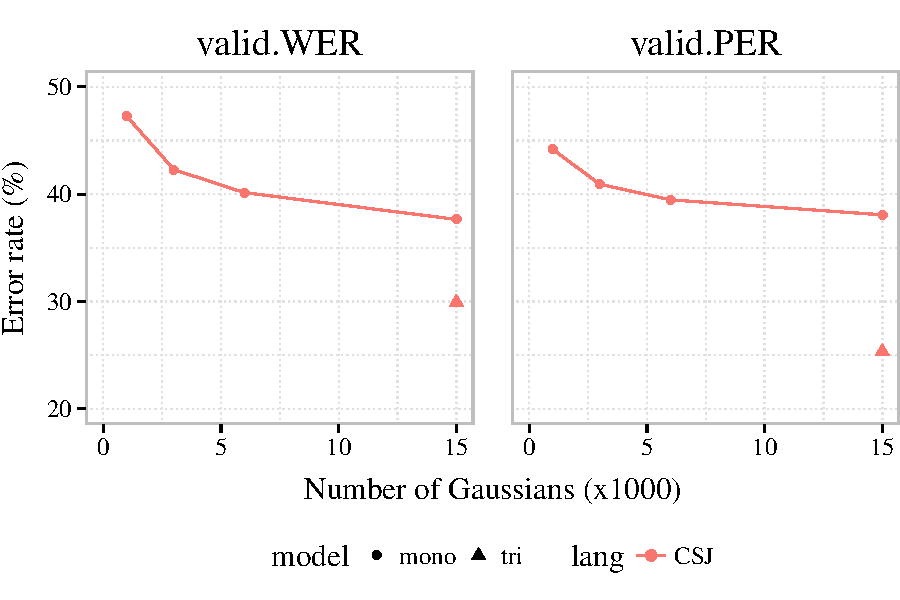
\includegraphics[trim={0 0 0 0}, clip, width=0.8\linewidth]{chapter03/ch3_misc_plotting/figures/plot_hmm_evaluations.pdf}
\caption{\textit{Changes in word error rate (\%WER) and phone error rate (\%PER) following variation of the number of total Gaussians allocated to monophone acoustic models (circles). The error rates obtained with a triphone model with $15,000$ Gaussians are included as comparison (triangles). Scores correspond to decoding performed on the validation set (i.e., unseen speakers for the CSJ and KCSS; already seen speakers for the WSJ).}}
\label{fig:hmm_gaussians}
\end{figure}


We tested the decoding performance on the validation set of AMs with total number of Gaussians going from $1,000$ to $15,000$. These values are used as default total number of Gaussians when training, respectively, monophone and triphone models in Kaldi (without speaker adaptation).
In order to do so, we used the language models described in section \ref{hmm_lm}, namely a word bigram LM and a phone unigram LM, which were used to obtain word error rates (\%WER) and phone error rates (\%PER), respectively. Note that while we provide word bigram WER\% as a reference value to compare with existing speech recognition models\footnote{As a reference, in 2015 some state-of-the-art speaker adapted HMM-GMM systems trained on 82 hours of the WSJ achieved $6.3\%$ WER \cite{panayotov2015} and $5.4\%$ WER \cite{chan2015} on the WSJ eval'92 dataset. Contemporary deep neural network-based systems achieved $3.5\%$ WER on the same dataset \cite{chan2015}.}, our main focus is on PER\%. Indeed, we will use our models in paradigms involving phonetic decoding of non-native nonwords; the phone unigram PER\% evaluation gives us an insight into how well our ASR systems can do phonetic decoding on native (non)words. 

As seen in Figure \ref{fig:hmm_gaussians}, we find that the performance of our models increased (i.e., error rates decreased) when increasing the number of total Gaussians from the Kaldi default of $1,000$ to $15,000$, which would average to approximately $125$ Gaussians per state for a language with an inventory of 35 phonemes\footnote{Phoneme counts: CSJ: 37, KCSS: 36, WSJ: 39}.   
Therefore, the acoustic models with the highest amount of Gaussians (i.e., $15,000$) give the best performance for monophone models, both at the lexical (\%WER) and phonetic (\%PER) levels of decoding.
We did not pursue increasing the number of Gaussians even further, as performance gain was reaching an asymptote at this point and adding more Gaussians would have increased the computational demands for each experiment. Additionally, we expect that adding ``too many'' Gaussians might have lead to overfitting of the models to the training set.
As expected, triphone models performed better than monophone models at phonetic decoding (\%PER), in spite of having the same amount of total Gaussians than our best monophone models (CSJ: $37.96\%$ monophone \textit{vs.} $25.33\%$ triphone; KCSS: $50.70\%$ monophone \textit{vs.} $38.42\%$ triphone). Later in this chapter we will discuss how it might be possible to increase acoustic model performance in future work, without having recourse to triphone HMMs, which as explained previously are not appropriate for our experiments.  

Concerning the test set (i.e., $15\%$ of the corpora), we find \%WER comparable to those obtained for the validation set (CSJ: $37.48\%$ on test, $37.64\%$ on validation; KCSS: $73.35\%$ on test, $74.03\%$ on validation), and similarly for \%PER (CSJ: $37.96\%$ on test, $38.07\%$ on validation; KCSS: $50.70\%$ on test and validation).
Since the validation and test sets contain utterances from the same speakers, this information does not allow us to evaluate our models' sensitivity when decoding data from speakers not used in the training data (recall that none of our models have any speaker adaptation; only CMVN is applied when processing the features). However, the fact that validation and test set scores are similar indicates that, while rudimentary, our acoustic models give stable performances when confronted with datasets with structurally different lexical exemplars and acoustically different phonetic exemplars.   

{\color{red}[TODO]: Add WSJ}
%> d.eval
%   corpus model totgauss   set   WER   PER
%1     CSJ  mono        1 valid 47.24 44.16
% 2     CSJ  mono        3 valid 42.28 40.92
% 3     CSJ  mono        6 valid 40.14 39.47
% 4     CSJ  mono       15 valid 37.64 38.07
% 5     CSJ   tri       15 valid 29.94 25.33
% 6     CSJ  mono       15  test 37.48 37.96

% 7    KCSS  mono        1 valid 81.39 56.23
% 8    KCSS  mono        3 valid 77.20 53.05
% 9    KCSS  mono        6 valid 75.59 51.66
% 10   KCSS  mono       15 valid 74.03 50.70
% 11   KCSS   tri       15 valid 65.48 38.42
% 12   KCSS  mono       15  test 73.35 50.70

% 13    WSJ  mono        1 valid 18.54    NA
% 14    WSJ  mono        3 valid 14.55    NA
% 15    WSJ  mono        6 valid 12.81    NA
% 16    WSJ  mono       15 valid 11.26    NA
% 17    WSJ   tri       15 valid  8.48    NA
% 18    WSJ  mono       15  test 11.50    NA

%%%%%%%%%%%%%
% SurfPhono %
%%%%%%%%%%%%%
\newpage
\section{Investigating the role of surface phonotactics} \label{3-surfphono}

\small{\textit{{\color{red}ADD ACKNOWLEDGEMENTS THOMAS + EMMANUEL.\\}}}

\subsection{Introduction}

%%% Background
In the previous section we described an ASR-based implementation of one-step models of nonnative speech perception, as described by \cite{dupoux2011, wilson2014}. In these models, nonnative speech perception is a process of reverse inference; the resulting percept is the output of a process where acoustic and phonotactic match are simultaneously optimised. \cite{wilson2014} formalises the reverse inference process as shown in equation \ref{eq_onestep2_ch3}, where $w$ corresponds to candidate percepts and $X$ corresponds to the stimulus acoustics.

\begin{equation}
  \widehat{w} = \underset{w}{arg\,max} \left \{ P(X|w) \cdot P(w) \right \}
  \label{eq_onestep2_ch3}
\end{equation}

Applying the ASR nomenclature, this equation can be paraphrased as follows: in one-step proposals, the resulting percept is the one that maximizes the product between the acoustic match $P(X|w)$, determined by an acoustic model (AM), and the phonotactic probability  $P(w)$, which is determined by a language model (LM).
While the optimisation process combines the probabilities given by the AM and LM, the two modules remain independent from one another before their product is computed. As such, it is possible to modify them in order to study their respective influences in the perception process.   

%%% Research question
As a continuation of our work on exemplar models in sections \ref{2-parlato} and \ref{2-parlato-dur}, a question that first arises is whether the output of the LM, namely the influence of phonotactics, is at all needed to explain the phenomenon of vowel epenthesis. We found in chapter \ref{chapter02} that acoustic information, such as vowel coarticulation, was essential in determining epenthetic vowel quality. One could hypothesize that the insertion of a vowel (as opposed to no insertion) is determined by how the acoustic cues are interpreted.

For instance, Japanese speakers can sometimes produce devoiced high vowels as a fricative vowel\footnote{Also referred to as a syllabic fricative} when they are preceded by a fricative consonant. In other words, the devoiced vowel becomes a prolongation of the fricative consonant, yet keeping articulatory and spectral information corresponding to the intended vowel \cite{matsui2017}\footnote{We thank Yasuyo Minagawa and Shigeto Kawahara for this comment.}. One could thus hypothesize that a fricative vowel is an acceptable allophone (i.e., model or exemplar) of vowels \textipa{/i/} or \textipa{/u/} in Japanese, while it is not in another language such as English, where the signal will be interpreted as a fricative instead. In this case, the difference in the interpretation of the same acoustic information could lead to epenthesis in Japanese but not in English. In a similar fashion, English listeners may interpret releases of stop consonants as reduced vowels, resulting in increased rates of epenthesis with increased release duration \cite{wilson2014}. 

However, are epenthetic repairs not due to cases of phonotactic illegality in the first place? Not necessarily. Indeed, Japanese listeners have been shown to perceive epenthetic vowels after certain acoustic realisations of coda \textipa{[n]}, even though this syllabic structure is phonotactically legal in Japanese. In loanword data, word-final \textipa{[n]} is adapted differently according to the language of origin of the word; French \textipa{/n/} may result in vowel epenthesis, becoming \textipa{[n:u]} or \textipa{[nu]} (e.g., \textit{Cannes} \textipa{/kan/} $\rightarrow$ \textipa{/kan:u/}) while English \textipa{[n]} is kept as a nasal coda consonant (e.g., \textit{pen} adapted as \textipa{/pen/}). This assymetry was observed in online perception with nonwords (therefore excluding the influence of orthography) and can be explained by the presence of a strong vocalic release in French \textipa{[n]} but not English \textipa{[n]} \cite{peperkamp2008}.
Also, an identical segmental structure might ellicit different amounts of epenthesis depending on the stimulus acoustics. An illustration from production is given by the imitation study on English listeners by \cite{wilson2014}. In that study, a cluster such as \textipa{/bn/}, which is phonotactically illegal in English, ellicited lower rates of epenthesis in one item (\textit{bnase}, $33\%$ epenthesis) than in another (\textit{bnapa}, $80\%$ epenthesis). The authors observed a correlation between the variability of certain acoustic cues in the target stimuli and the variability in the rates of epenthesis (and other errors such as prothesis and consonant deletion) in production.

%%% What & How
In this section we investigate the hypothesis stating that acoustic match is sufficient to account for epenthetic patterns in nonnative speech. To do so, in a first step, we compare the performance, relative to human data, of ASR models that share the same AM but differ in the LM used during decoding. Notably, we assess if LMs with basic phonotactic information better approximate human behaviour than a null LM. In a second step, we assess if the best AM-LM combination is capable of mirroring qualitative effects observed in human data.
%%% Plan
As reference, we use psycholinguistic data from the identification tasks described in section \ref{2-ahpa} (Experiment 1) and section \ref{2-parlato} (Experiment 2). 


\subsection{Experiment 1}%: {\color{red}m-/ahpa/}}
In this experiment we investigated how various versions of our ASR model differing in their language models (LMs) compared to real behavioural data. While we varied the LMs, the acoustic model was kept constant; as stated in the previous section, we used HMM-GMM monophone models with $15000$ Gaussians. We used our models to perform simulations of the identification task described in section \ref{2-ahpa}, where Japanese listeners were asked to indicate whether they heard an epenthetic vowel within the consonant cluster of $V_{1}C_{1}C_{2}V_{1}$ items (e.g., \textipa{/ahpa/}). For these items, the quality of the coarticulation cues either matched or mismatched the quality of the flanking vowels. We analysed the results quantitatively in order to assess if injecting additional phonotactic information allowed the model to better approximate human responses. We also performed qualitative analyses in order to see if the best version of the model reproduced the effects observed in section \ref{2-ahpa}. 

\subsubsection{Methods}
\paragraph{Stimuli}
We used the same stimuli as in section \ref{2-ahpa}. As a reminder, we recorded 3 speakers producing disyllabic $V_{1}C_{1}C_{2}V_{1}$ and trisyllabic $V_{1}C_{1}V_{2}C_{2}V_{1}$, with $V_{1}$ a flanking vowel in the set \textipa{/a, e, i, o, u/}, $C_{1}$ \textipa{/h/} or /k/, and $C_{2}$ a fixed consonant, /p/ (e.g, \textipa{/ahpa/}, \textipa{/ahapa/}). By cross-splicing the disyllabic natural control items (e.g., \textipa{/ahpa/}), we obtained disyllabic spliced control items (e.g., \texorpdfstring{\textipa{/ah\textsubscript{a}pa/}}{}), disyllabic spliced test stimuli (e.g., \texorpdfstring{\textipa{/ah\textsubscript{u}pa/}}{}), and trisyllabic spliced fillers (e.g., {\textipa{/ahapa/}), where subscripts indicate the identity of the vowels flanking the clusters in the original recording. Therefore, within each speaker, all stimuli of the same structure (in our example, \textipa{/ah($V$)pa/} items) have acoustically identical flanking vowels.
  
\paragraph{Language models}
In order for the decoding task to be analogous to the behavioural experiment described in section \ref{2-ahpa}, trial-specific language models were constructed, as shown in Figure \ref{fig:m-ahpa_G}. Thus, when decoding a $V_{1}C_{1}(V_{2})C_{2}V_{1}$ stimulus, the perception model was only given the possibility to transcribe it as $V_{1}C_{1}(V_{2})(SIL)C_{2}V_{1}$, where phones between parentheses are optional, $V_{2}$ was from the set of vowels \textipa{/a, e, i, o, u/}, and $SIL$ is an optional silence\footnote{$SIL$, which corresponds to the closure of the plosive \textipa{/p/}, is added in order to reduce alignment artifacts. Additionally, it allows us to also model the alternative parsing of the items as a sequence of two nonwords.}. 

\begin{figure}[htb]
    \centering
    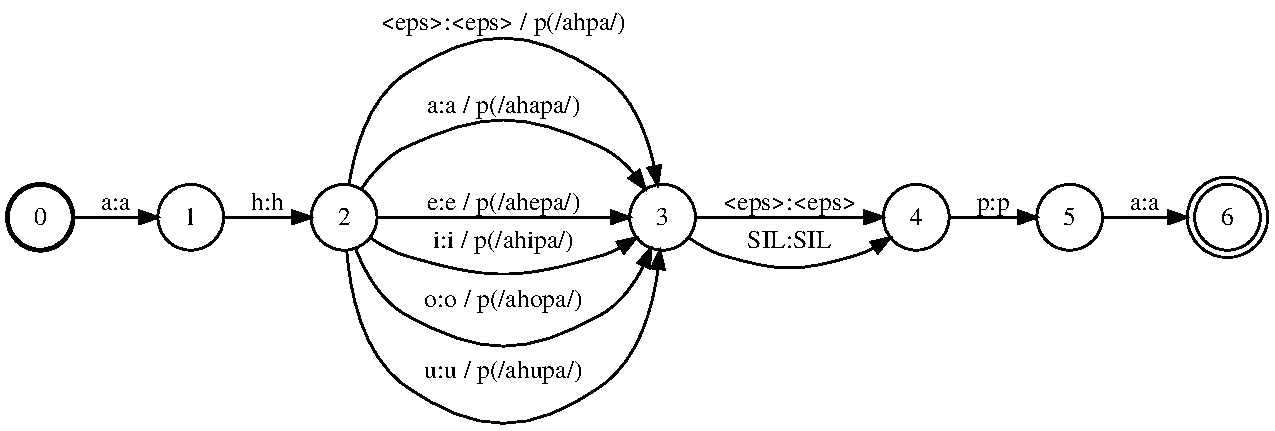
\includegraphics[width=0.8\linewidth]{chapter03/m-ahpa_Gfst.pdf}
    \caption{\textit{Constrained language model used to test the models (here: LM for \textipa{/ahpa/} trials). Nodes in the graph represent states, weighted edges represent transitions between states (here: phonemes). When relevant, weighted edges are labeled with the probability to choose that edge when decoding, which affects the final language model score of each possible path. When no weights are shown (e.g., between states 3 and 4), there is no preference between the paths concerned. The language model scores are combined with acoustic scores when decoding experimental items.}}
    \label{fig:m-ahpa_G}
\end{figure}

In this section, we investigate the type of phonotactic information that might be used by Japanese listeners when perceiving foreign speech that does not conform to native phonotactics. We test 5 types of language models (LM) when decoding our $V_{1}C_{1}(V_{2})C_{2}V_{1}$ items; these LMs differ only in the weights given to edges between nodes 2 and 3 in the graph shown in Figure \ref{fig:m-ahpa_G}. The weights were obtained by computing frequency counts from the portion of the CSJ used for training the acoustic model. Using the same acoustic model, we compared the following LMs {\color{red}[TODO] Add formulae as annex}: 

\begin{enumerate}
    \item A null LM, which implies that listeners base their decoding of consonant clusters on phonetic match alone, without using information on phonotactics.
    \item A phone-unigram LM, which implies that listeners do not take neighbouring phonemes into consideration when decoding the consonant clusters; only the frequency of the vowel $V_{2}$ to be epenthesized (compared to that of $C_{2}$) is taken into account when choosing epenthetic vowel quality.
    \item An online phone-bigram language model, which implies that listeners decode the clusters as they hear them (i.e., decoding is done from the start of the item), and the choice of (no) vowel is conditioned on the presence of $C_{1}$. Therefore, the choice of epenthetic vowel is modulated by $C_{1}V_{2}$ and $C_{1}C_{2}$ diphone frequencies. 
    \item A retro phone-bigram language model, which implies that listeners decode the clusters based on the most recent information (i.e., decoding is done from the end of the item), and the choice of (no) vowel is conditioned on the presence of $C_{2}$. Thus, the choice of epenthetic vowel is modulated by $V_{ep}C_{2}$ and $C_{1}C_{2}$ diphone frequencies.
    \item A batch phone-bigram language model, which implies that listeners decode the item considering the entire structure, taking into consideration the probability of having a vowel $V_{2}$ given the presence of $C_{1}$ and $C_{2}$. Here the choice of epenthetic vowel is modulated by the product of $C_{1}V_{2}$ and $V_{2}C_{2}$ (or by $C_{1}C_{2}$) diphone frequencies.  
\end{enumerate}
    
\paragraph{Identification task simulation}
\begin{figure}[htb]
  \centering
  \begin{overpic}[trim={0 1cm 0 1.5cm},clip, width=0.7\linewidth]{chapter03/m-ahpa_praat_ah0apa.pdf}\end{overpic}
  \caption{\textit{Example of how the ASR system decodes the item \textipa{/ah$_{a}$pa/}, using the null version of the language model in Figure \ref{fig:m-ahpa_G}. From top to bottom: original waveform, item name, aligned transcriptions given by the model (from the most probable to the least probable, with the corresponding posteriorgrams shown to their right side), and spectrogram with formant contours. SIL = silence. {\color{red}TODO: get updated figure (this is with mono-6K); ALSO: change item name to phonemic transcription}}}
  \label{fig:m-ahpa_align}
\end{figure}

After decoding the stimuli, we extracted from the resulting lattice each possible transcription of each item, and the corresponding acoustic and language model scores. An example of how the ASR system decodes the experimental stimuli can be seen in Figure \ref{fig:m-ahpa_align}. From the (scaled) acoustic and language model scores we derived the item posteriorgrams, which indicate how probable a given transcription was given the audio input. We used these probabilities as proxies of the probability that a listener might exploit when performing reverse inference during speech perception, and therefore, the probabilities used when responding in an identification task. 

As such, for each item, we obtained a six-dimensional vector $ident_{model} = [p_{none}, p_{a}, p_{e}, p_{i}, p_{o}, p_{u}]$, containing a discrete probability distribution, with a probability mass function linking the identification task options `none', `a', `e', `i', `o', `u', to their respective probabilities (i.e., posteriorgrams).
We can define the human equivalent $ident_{human} = [p_{none}, p_{a}, p_{e}, p_{i}, p_{o}, p_{u}]$, which contains the percentage of responses for each item, after aggregating all participant responses. 

\subsubsection{Quantitative analysis}
In order to perform a global evaluation of the similarity between the behavioural responses and the responses obtained with the five LMs described above, we computed the Pearson's product-moment correlation coefficient between the human and model posteriorgrams. The model with the highest correlation to the human data was the \textsc{null} LM ($r = 0.76$), followed by the \textsc{unigram}, \textsc{bigram online}, and \textsc{bigram retro} LMs ($r = 0.65$), and lastly, the \textsc{bigram batch} LM ($r = 0.62$). Numerically, the \textsc{null} LM better approximated the human data.

In order to assess if the correlation differences between the \textsc{null} LM and other LMs were significant, we computed these differences and their corresponding 95\% confidence intervals (CIs), using bootstrapping with 1000 samples\footnote{Sampling was done by item.}. As can be seen in Table \ref{tab:m-ahpa-cor_diff}, the correlation between the human data and the output of the \textsc{null} LM was significantly higher than those of other LMs.

% latex table generated in R 3.3.3 by xtable 1.8-2 package
% Mon Jul  2 21:36:40 2018
\begin{table}[htb!]
\centering
\caption{\textit{Difference in correlation with human data between the null LM and other LMs. The lower and upper bounds of the 95\% confidence intervals are given between brackets. Positive values indicate higher correlation between human data and null model output than between human data and other LM output.}}
  \label{tab:m-ahpa-cor_diff}
\vspace{0.25cm}
\begin{tabular}{lccc}
  \toprule
 & Correlations & Difference & Significant? \\  \midrule
null vs. unigram & $0.76 - 0.65$ & $0.10$ $[0.07, 0.14]$ & Yes \\ 
  null vs. bigram online & $0.76 - 0.65$ & $0.11$ $[0.08, 0.14]$ & Yes \\ 
  null vs. bigram retro & $0.76 - 0.65$ & $0.10$ $[0.07, 0.13]$ & Yes \\ 
  null vs. bigram batch & $0.76 - 0.62$ & $0.13$ $[0.10, 0.17]$ & Yes \\ \bottomrule 
\end{tabular}
\end{table}

Contrary to the null and unigram LMs, the bigram models were subject to an arbitrarily set smoothing parameter, which determined the probability of choosing a sequence of phonemes that had never been observed in the training data. We set this smoothing parameter to $10^{-8}$, which is a strict value, as it is relatively close to zero. This was done in order to evaluate whether the acoustic match could rescue decoding options which are not supported by the language's phonotactics. In order to evaluate the similarity between models' outputs and human data without the influence of the value of the smoothing parameter, we computed the correlation between the human data and models' posteriorgrams after excluding the posteriorgrams for ``none'' responses and re-normalising the remaining posteriorgrams. As such, we are focusing on the correlation related to epenthetic vowel quality.
Here, the highest correlation still corresponded to the \textsc{null} LM ($r = 0.77$), followed by the \textsc{bigram retro} ($r = 0.74$), the \textsc{bigram online} ($r = 0.73$), and finally the \textsc{unigram} and the \textsc{bigram batch} LMs ($r = 0.71$). 
As shown in Table \ref{tab:m-ahpa-cor_diff-nonone}, while the difference between the correlations diminished relative to what is shown in Table \ref{tab:m-ahpa-cor_diff}, the CIs still did not overlap with zero, meaning that the correlation between the human data and the output of the \textsc{null} LM was significantly higher than those of other LMs.  

% latex table generated in R 3.3.3 by xtable 1.8-2 package
% Tue Jul  3 03:37:50 2018
\begin{table}[htb!]
\centering
\caption{\textit{Difference in correlation with human data between the null LM and other LMs, after removing the ``none'' responses. The lower and upper bounds of the 95\% confidence intervals are given between brackets. Positive values indicate higher correlation between human data and null model output than between human data and other LM output.}}
\label{tab:m-ahpa-cor_diff-nonone}
\vspace{0.25cm}
\begin{tabular}{lccc}
   \toprule
  & Correlations & Difference & Significant? \\  \midrule
  null vs. unigram & $0.77 - 0.71$ & $0.05$ $[0.03, 0.08]$ & Yes  \\  
  null vs. bigram online & $0.77 - 0.73$ & $0.04$ $[0.02, 0.06]$ & Yes \\   
  null vs. bigram retro & $0.77 - 0.74$ & $0.02$ $[0.01, 0.04]$ & Yes \\ 
  null vs. bigram batch & $0.77 - 0.71$ & $0.06$ $[0.03, 0.08]$ & Yes \\ \bottomrule 
\end{tabular}
\end{table}

\subsubsection{Qualitative analyses}

\paragraph{Identification accuracy}
Using the set of filler items such as \textipa{/ahapa/} and \textipa{/okipo/} (i.e., spliced items with a full vowel between $C_1$ and $C_2$), we can assess identification accuracy relative to our item labels. Indeed, recall that while our phonetically-trained speakers were instructed to read items following ``standard'' IPA pronunciations, it is possible for our human participants to not perceive the intended vowel categories due to adaptation processes (e.g., misperceiving \textipa{/u/}, which is not realised as \textipa{[u]} but as \textipa{[W]} in Japanese), and/or due to speaker idiosyncrasies.

\begin{figure}[htb]
\centering
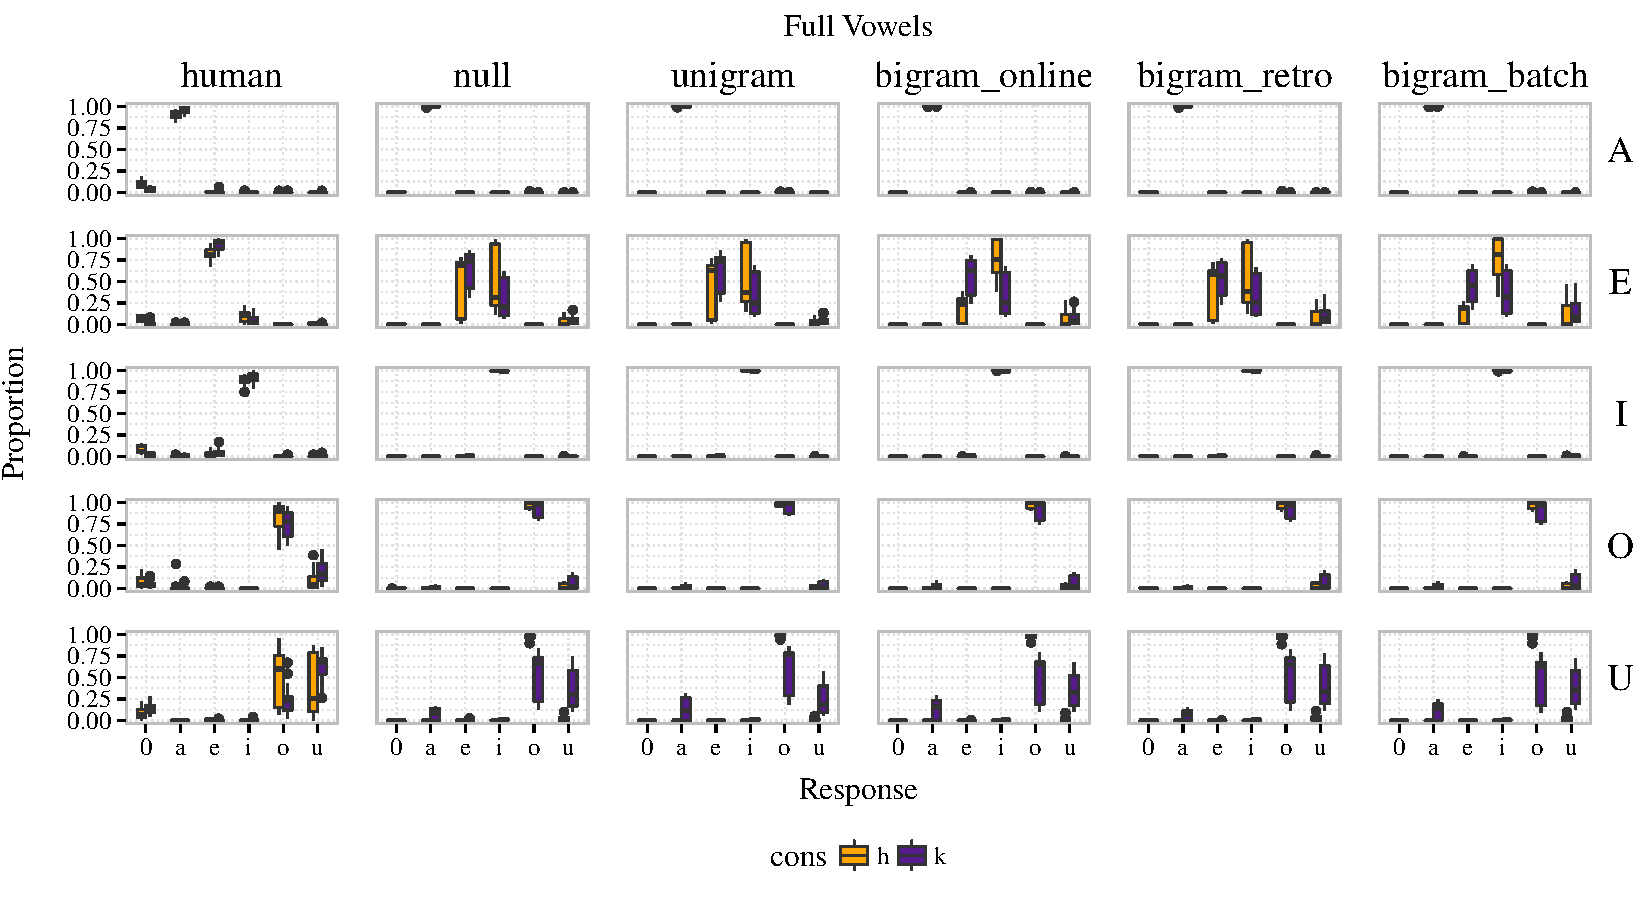
\includegraphics[width=1\linewidth]{chapter03/m-ahpa_figures.pdf}
\caption{\textit{Response patterns for the identification task on full vowel stimuli (filler items). Human and models responses are separated by columns; intended identity of the medial vowel is given by rows. Within each rectangle, the horizontal axis corresponds to possible responses from the set \{``none'', ``a'', ``e'', ``i'', ``o'' , ``u''\}. The vertical axis corresponds to proportion of responses (i.e., posteriorgrams, in the case of models). The box and whiskers plots display the distribution of the proportions across items (median, quartiles and extrema). For instance, we can see from the first row that, similar to humans, all models correctly classified most /VC\textipa{ap}V/ items as containing a medial \textipa{/a/} vowel.}}
\label{fig:m-ahpa_fV_acc}
\end{figure}

%Distribution of the proportion of responses given by human participants (leftmost panels) and posteriorgrams obtained when decoding with different language models. The box and whiskers plots display the distribution of posteriorgrams across experimental items, with boxplots separated according to the $C_{1}$ in the cluster and the responses (rows).

Overall, human participants identified the correct intended vowel category in $79.5\%$ of the trials. As can be seen in Figure \ref{fig:m-ahpa_fV_acc}, this was mostly due to confusions between the intended \textipa{/o/} and \textipa{/u/} categories, with most errors consisting of \textipa{/u/} being identified as \textipa{/o/}.
Consistent with our correlation analyses, the \textsc{null} LM gave the highest accuracy out of all models (accuracy: $74\%$), followed by the \textsc{bigram retro} (accuracy: $72.6\%$), the \textsc{unigram} (accuracy: $72.5\%$), the \textsc{bigram online} (accuracy: $72.6\%$), and finally the \textsc{bigram batch} LM (accuracy: $68.7\%$). 
As seen in Figure \ref{fig:m-ahpa_fV_acc}, like human participants, the models showed difficulty categorising \textipa{/u/} items as such; in particular, these were almost always classified as exemplars of \textipa{/o/} when $C_2 = \textipa{/h/}$. However, unlike human participants, models misperceived \textipa{/e/} as \textipa{/i/}. This misperception appears to be worse for the \textsc{bigram online} and \textsc{bigram batch} language models.
In sum, while the accuracy rates for the models were close to that of humans, we saw that the models showed not only quantitative but also qualitative differences in their identification of non-native full vowels, in comparison with human participants. Below we continue our qualitative analyses on what was determined to be the best model according to the correlation analyses and the filler item accuracy, namely the ASR system with a \textsc{null} LM.  

\paragraph{Control items}
Human participants experienced vowel epenthesis in $56\%$ (\textipa{/hp/}: $52\%$; \textipa{/kp/}: $61\%$)\footnote{Note that since posteriorgrams are computed by weighting items from all three speakers equally, values reported in this section might differ slightly from those in section \ref{2-ahpa}. Indeed, due to how data was cleaned in section \ref{2-ahpa}, some trials were removed and the number of trials per item per speaker might have differed in some cases. In order to ensure that human and model data are comparable, we re-do statistical analyses of human data when necessary and report the resulting coefficients.} of control items in which the flanking vowel and coarticulation are of the same quality. The \textsc{null LM} gave an output of $68\%$ epenthesis, with $72\%$ and $65\%$ epenthesis for \textipa{/hp/} and \textipa{/kp/}, respectively. As such, the model gave a higher percentage of epenthesis for \textipa{/hp/} clusters compared to \textipa{/kp/}clusters, while the opposite was true for humans.

Now we focus on epenthetic vowel quality, meaning that we perform analyses after removing ``none'' responses and re-normalising posteriorgrams. We find that, like humans (\textipa{/hp/}: $44\%$; \textipa{/kp/}: $87\%$; total: $66\%$), the model gave lower percentages of default \textipa{/u/}-epenthesis for \textipa{/hp/}- ($47\%$) than for \textipa{/kp/}- ($65\%$) clusters (total: $56\%$). However, this difference is not as marked as it is for Japanese listeners. Recall that in section \ref{2-ahpa} we found that Japanese listeners experience significantly more default \textipa{/u/}-epenthesis for \textipa{/kp/} clusters, and significantly more vowel copy epenthesis for \textipa{/hp/} clusters. These patterns of responses mirrored loanword data. Do we find these effects in the output of our model? 

We first examined possible effects of consonant cluster on default \textipa{/u/}-epenthesis by using the R statistical software \cite{R-base}, using Markov chain Monte Carlo generalised linear mixed-models \cite{R-MCMCglmm, R-coda}. These Bayesian models sample coefficients from the posterior probability distribution conditioned on the data and given priors. We used priors that are standard for linear models. Model convergence was assessed by visual inspection of trace plots and the Gelman–Rubin convergence diagnostic \cite{gelman1992}, using eight chains with different initialisations. Effects were considered statistically significant if the 95\% highest posterior density (HPD) interval estimated for the coefficient of interest did not include zero. We report both the posterior mode and the 95\% HPD interval.  

The left panel of Figure \ref{fig:m-ahpa_ctrl} shows the posteriograms of \textipa{/u/}-epenthesis for humans and all models. For the ASR system with the null LM, we assessed the variation of the continuous response variable ``u'' response \textsc{Posteriorgram} that was caused by the fixed effect \textsc{Consonant} cluster (\textipa{/kp/} \textit{vs.} \textipa{/hp/}; contrast coded with deviance coding).
We initially included random intercepts for \textsc{Speaker} and \textsc{Item}, as well as a random slope for \textsc{Speaker} on \textsc{Consonant}. However, these were removed as their addition caused the models to be singular (estimated null variances), with consequently poor trace plots.
We found the main effect of \textsc{Consonant} to be significant (mode: $-0.19$, HPD: $[-0.29,-0.07]$), meaning that as for humans (mode: $-0.42$, HPD: $[-0.61,-0.26]$), the model gave significantly more \textipa{/u/}-epenthesis for \textipa{/hp/}- than for \textipa{/kp/}-clusters. However, as evidenced by the statistical model coefficients, the magnitude of the effect is larger for humans than for the model.  

\begin{figure}[htb]
\centering
\includegraphics[page=8, width=1\linewidth]{chapter03/m-ahpa_figures.pdf}
\caption{\textit{Proportion of default \textipa{/u/}-epenthesis (left) and vowel copy epenthesis (right) given by human participants and models. The box and whiskers plots display the distribution of the proportions across items (median, quartiles, extrema and outliers).}}
\label{fig:m-ahpa_ctrl}
\end{figure}

Turning to vowel copy epenthesis in control items for which the flanking vowel was not \textipa{/u/}, we used the same statistical models but with copy vowel \textsc{Posteriorgram} as the continuous response variable. For instance, for the item \textipa{/ek$_{e}$pe/}, this was the posteriorgram for the ``e'' response. The distribution of posteriorgrams for humans and all models is shown in the right panel of Figure \ref{fig:m-ahpa_ctrl}.
While there was a trend in the same direction for the null LM, namely higher percentages of vowel copy for \textipa{/hp/}- than for \textipa{/kp/}-clusters, we did not find a significant main effect of \textsc{Consonant} for the model (mode: $0.11$, HPD: $[-0.02, 0.24]$) as we did for humans (mode: $0.39$, HPD: $[0.20, 0.58]$). 

\paragraph{Test items}
Next we examine the identification task response patterns for test items. As a reminder, for these spliced items, the vowel coarticulation was different from the flanking vowels.

\begin{figure}[htb!]
\centering
\includegraphics[page=5, width=0.9\linewidth]{chapter03/m-ahpa_figures.pdf}
\caption{\textit{Response patterns for the identification task on spliced test stimuli. Horizontal axes correspond to possible responses from the set \{``none'', ``a'', ``e'', ``i'', ``o'' , ``u''\}. Vertical axes correspond to proportion of responses (i.e., posteriorgrams, in the case of models). The box and whiskers plots display the distribution of the proportions across items (median, quartiles, extrema, and outliers).}}
\label{fig:m-ahpa_test_coll}
\end{figure}

As shown in Figure \ref{fig:m-ahpa_test_coll}, reponses that were represented the most in the null model posteriorgrams were {\color{red}``none'' (\%), ``i'' (\%), and ``u'' (\%)}. These were also the responses that human participants gave the most {\color{red}(``none'' (\%), ``i'' (\%), and ``u'' (\%))}.

We saw in section \ref{2-ahpa} that, for human participants, responses were mainly determined by the quality of the vowel coarticulation within the consonant cluster. This manifested itself in the appearance of horizontal bars, and some very faint vertical bars, in the top panels of Figure \ref{fig:m-ahpa_test_heat}. Do we observe something similar in the output of the model with null LM?

\begin{figure}[htb!]
\centering
\includegraphics[page=9, width=0.9\linewidth]{chapter03/m-ahpa_figures.pdf} \\ \vspace{0.5cm}
\includegraphics[page=10, width=0.9\linewidth]{chapter03/m-ahpa_figures.pdf}
\caption{\textit{Counts of responses for the test items for human participants (top panel) and the ASR model with a null LM (bottom panel). Within each panel: Top: \textipa{/hp/-}items; bottom: \textipa{/kp/-}items. Within each rectangle, flanking vowels and vowel coarticulation are given in the horizontal and vertical axes, respectively. Darker colours indicate higher counts. Concerning human data, only test items are included here, while the very similar Figure \ref{fig:tiles} from section \ref{2-ahpa} includes test items, as well as spliced control items.}}
\label{fig:m-ahpa_test_heat}
\end{figure}

When examining the bottom panels in Figure \ref{fig:m-ahpa_test_heat}, we see that response patterns are noisier than for human participants. In spite of that, we can notice several similarities to human responses.
We generally see that responses are mostly organised in horizontal lines, with ``none'' and ``u'' responses spread relatively uniformly across all combinations of vowel coarticulations and flanking vowels. This spread was even more uniform than for human responses, where less ``u'' responses were given for items with front vowel coarticulation (i.e., \textipa{[i, e]}). In spite of this increase in ``u'' responses for items with front vowel coarticulation, the model responses show that, as for humans, most ``i'' responses were triggered by front vowel coarticulation.

When focusing on \textipa{/hp} items, we see that for human responses there is a correspondence between the quality of the vowel coarticulation and the response (e.g., most ``a'' responses come from items with \textipa{[a]} coarticulation). This correspondence is blurred in the model responses, as follows:
\begin{itemize}
    \item ``a'' responses: A horizontal line is visible corresponding to \textipa{[a]} vowel coarticulation as it is for human responses. However, additional horizontal lines corresponding to back vowel coarticulation (i.e., \textipa{[o, u]}) are also visible. The source of most ``a'' responses are items with \textipa{[u]} coarticulation.
    \item ``e'' responses: These were triggered by front vowel coarticulation for the model, while for humans they were triggered specifically by \textipa{[e]} vowel coarticulation (horizontal line) and \textipa{/e/} flanking vowel (fainter vertical line).
    \item ``i'' responses: Similar to humans, the majority of ``i'' responses given by the model were triggered by front vowel coarticulation. However, instead of seeing fainter vertical lines corresponding to front vowel flanking vowels as in human responses, for the model, ``i'' responses were also triggered to a lesser extent by non-front vowel coarticulation, even when the flanking vowel was not a front vowel.
    \item ``o'' responses: For humans, this response was triggered by back vowel coarticulation. For the model, \textipa{[a]} vowel coarticulation also triggered ``o'' responses. In other words, ``o'' responses were mostly triggered by non-front vowel coarticulation.
  
  \end{itemize}

  Additionally, we see that differences between model responses for \textipa{/hp/}-items and \textipa{/kp/}-items is not as apparent as it is for human responses. In the latter (top panels of Figure \ref{fig:m-ahpa_test_heat}), we see that participants barely responded \{``a'', ``e'', ``o''\} for \textipa{/kp/}-items. Meanwhile, for model responses, the rectangles for \{``a'', ``e'', ``o''\} responses for \textipa{/kp/}-items are fainter versions of their \textipa{/hp/} counterparts.
  
  Results from section \ref{2-ahpa} led us to conclude that vowel coarticulation, which was less present in \textipa{/kp/} clusters, influenced response patterns less for \textipa{/kp/}-items than for \textipa{/hp/}-items.
  Coherent with qualitative analyses on vowel copy epenthesis in control items, the difference of the effect of vowel coarticulation on \textipa{/hp/}- and \textipa{/kp/}-items is not as marked for the model as it is for human participants. 

% \begin{figure}[htb!]
% \centering
% \includegraphics[page=4, width=1\linewidth]{chapter03/m-ahpa_figures.pdf}
% \caption{\textit{Response patterns for the identification task on spliced test stimuli. Human and models responses are separated by columns; vowel coarticulation within the consonant clusters is given by rows. Within each rectangle, the horizontal axis corresponds to possible responses from the set \{``none'', ``a'', ``e'', ``i'', ``o'' , ``u''\}. The vertical axis corresponds to proportion of responses (i.e., posteriorgrams, in the case of models). The box and whiskers plots display the distribution of the proportions across items (median, quartiles and extrema).}}
% \label{fig:m-ahpa_test}
% \end{figure}

\subsubsection{Summary}
In summary, through quantitative analyses, we found that, out of the different LM tested, the responses from the ASR model with a null LM better approximated human responses. Qualitative analyses showed that the null LM model responses where generally similar to human responses, but with some twists.

For the identification of full vowels, like humans, the model was accurate at identifying \textipa{/a, i, o/}. Like humans, the model identified \textipa{/u/} as ``o'' in many instances; however, the specific patterns were not exactly mirroring the confusions observed in human responses. Also unlike humans, the model identified instances of \textipa{/e/} as ``i''.

For the identification of control items (i.e., spliced items with matching vowel coarticulation and flanking vowel), the model numerically mirrored the two effects observed in human responses: more default \textipa{/u/} epenthesis for \textipa{/kp/}-items than \textipa{/hp/}-items, and more copy vowel epenthesis for \textipa{/hp/}-items than \textipa{/kp/}-items. However, the effects are damped for the model; the latter difference was not significant for the model, while the former was significant but of lower magnitude than in human responses. Also unlike humans, the model epenthesized vowels more often for \textipa{/hp/}-items than for \textipa{/kp/}-items, as the opposite was true for humans. 

Concerning the test items (i.e., spliced items with mismatching vowel coarticulation and flanking vowel), like humans, most of the null LM model responses are in the set \{``none'', ``u'', ``i''\}. When examining model responses more in detail, we found that vowel coarticulation was driving responses as for humans, but the influence was less specific. One thing to note is that the differences observed in the model responses do not appear to be random; they are in line with the acoustics of the stimuli. As seen in the acoustic analyses of the items in section \ref{2-ahpa}, vowel coarticulations in \textipa{/hp/}-items can be clustered as follows, based on their formant values: [[[a,u],o][e,i]]. There is a separation of front and non-front vowel coarticulations, which is also seen in the model responses. Since humans also seem to be sensitive to this acoustic proximity (e.g., ``i'' responses mostly triggered by \textipa{[i,e]} coarticulation; ``o'' responses mostly triggered by \textipa{[o,u]} coarticulation), a question that arises is if the noise observed in the model might be reduced when using a more performant acoustic model in the ASR system; indeed, we are not using state-of-the-art models (see below for further discussion). We will now present a similar analysis of the model's ability to model Japanese listeners' behaviour, performed on data from a different psycholinguistcs experiment.       

\subsection{Experiment 2}
As in the previous experiment, here we investigated how various versions of our ASR model differing in their language models (LMs) compared to real behavioural data.
The models were used to simulate the identification task described in sections \ref{2-parlato} and \ref{2-parlato-dur}, where Japanese listeners were asked to indicate whether they heard an epenthetic vowel within the consonant cluster of $V_{1}C_{1}C_{2}V_{2}$ items (e.g., \textipa{/abgi/}). For human participants, we saw that (1) they mostly experienced default \textipa{/u/}-epenthesis, and (2) the quality of the flanking vowels $V_{1}$ and $V_{2}$ modulated their responses due to coarticulation. Does the output of the ASR model that best approximated human responses reflected these two aforementioned effects? 

\subsubsection{Methods}
\paragraph{Stimuli}
We used the same stimuli as in sections \ref{2-parlato} and \ref{2-parlato-dur}. As a reminder, a native French speaker recorded 54 items with the structure $V_{1}C_{1}C_{2}V_{2}$, with $V_{1}$ and $V_{2}$ vowels from the set \{/a/, /i/, /u/\}, and $C_{1}C_{2}$ a cluster from the set \{/bg/, /bn/, /db/, /dg/, /gb/, /gn/\} (e.g. /abgi/).

\paragraph{Language models}

In order for the decoding task to be analogous to the behavioural experiment described in section \ref{2-parlato_per}, trial-specific language models were constructed, as shown in Figure \ref{fig:parlato_G}. Thus, when decoding a $V_{1}C_{1}C_{2}V_{2}$ stimulus, the perception model was only given the possibility to transcribe it as $V_{1}C_{1}(V_{ep})(SIL)C_{2}V_{2}$, where phones between parentheses are optional and $V_{ep}$ was from the set of vowels \textipa{/a, e, i, o, u/}, and $SIL$ is an optional silence. Concerning the weights between states 2 and 3, we created language models in a way analogous to the LMs in Experiment 1, adapted to the $V_{1}C_{1}C_{2}V_{2}$ items used in this experiment.

\begin{figure}[htb]
\centering
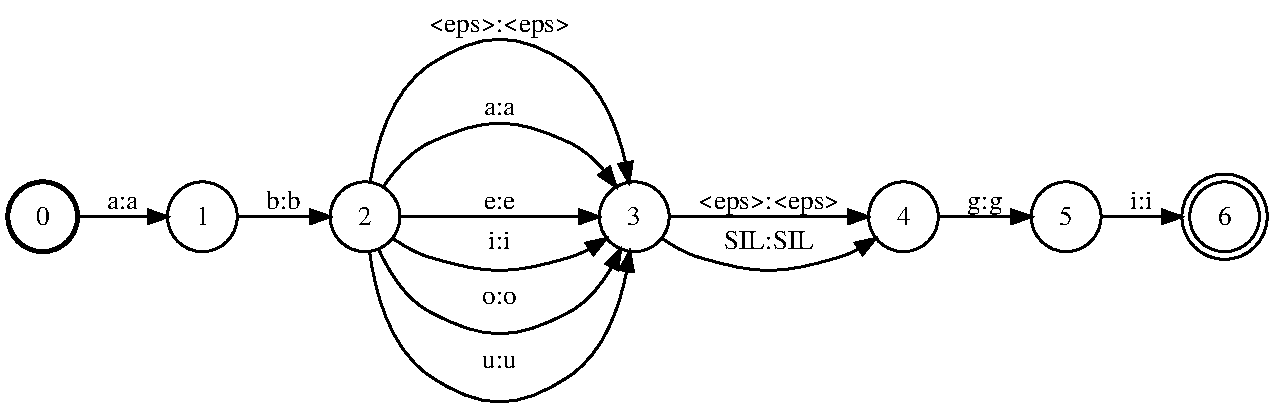
\includegraphics[width=0.8\linewidth]{chapter03/parlato_hmm_Gfst.pdf}
\caption{\textit{Constrained language model used to test the models (here: LM for decoding \textipa{/agni/}). Nodes in the graph represent states, weighted edges represent transitions between states (here: phonemes). When relevant, weighted edges are labeled with the probability to choose that edge when decoding, which affects the final language model score of each possible path. When no weights are shown (e.g., between states 3 and 4), there is no preference between the paths concerned. The language model scores are combined with acoustic scores when decoding experimental items.
}}
\label{fig:parlato_G}
\end{figure}

\paragraph{Identification task simulation}
We used the same procedure as in Experiment 1. An example of how the ASR system decodes the experimental stimuli can be seen in Figure \ref{fig:parl_hmm_align}. 

\begin{figure}[htb!]
  \centering
  \begin{overpic}[trim={0 2.5cm 0 1.5cm},clip, width=0.7\linewidth]{chapter03/parlato-hmm_praat_agni.pdf}\end{overpic}
  \caption{\textit{Example of how the ASR system decodes the item \textipa{/agni/}, using the null version of the language model in Figure \ref{fig:parlato_G}. From top to bottom: original waveform, item name, aligned transcriptions given by the model (from the most probable to the least probable, with the corresponding posteriorgrams shown to their right side), and spectrogram with formant contours. SIL = silence. {\color{red}TODO: get updated figure (this is with mono-6K)}}}
  \label{fig:parl_hmm_align}
\end{figure}

\subsubsection{Results: Quantitative analysis}
As in Experiment 1, we computed the Pearson's product-moment correlation coefficient between the human and model posteriorgrams in order to assess a global measure of the ressemblance between models' outputs and human data from section \ref{2-parlato_per}. The model with the highest correlation to the human data was the \textsc{bigram retro} LM ($r = 0.43$), followed by the \textsc{null} ($r = 0.40$), the \textsc{unigram} ($r = 0.30$), the \textsc{bigram online} ($r = 0.23$) and lastly, the \textsc{bigram batch} LM ($r = 0.19$). Numerically, the \textsc{bigram retro} LM better approximated the human data.

In order to assess if the correlation differences between the \textsc{null} LM and other LMs were significant, we computed these differences and their corresponding 95\% confidence intervals (CIs), using bootstrapping with 1000 samples. As can be seen in Table \ref{tab:parlato_lms-cor_diff}, the correlation between the human data and the output of the \textsc{null} LM was significantly higher than those of the \textsc{unigram}, \textsc{bigram online} and \textsc{bigram batch}. While the correlation to the human data for the \textsc{bigram retro} LM was numerically higher than for the \textsc{null} LM, we did not find evidence of a significant difference between the two as the CIs of their difference overlaps zero.

% latex table generated in R 3.3.3 by xtable 1.8-2 package
% Tue Jul  3 03:53:37 2018
\begin{table}[ht]
\centering
\caption{\textit{Difference in correlation with human data between the null LM and other LMs. The lower and upper bounds of the 95\% confidence intervals are given between brackets. Positive values indicate higher correlation between human data and null model output than between human data and other LM output.}}
\label{tab:parlato_lms-cor_diff}
\vspace{0.25cm}
\begin{tabular}{lccc}
   \toprule
  & Correlations & Difference & Significant? \\  \midrule
null vs. unigram & $0.40 - 0.30$ & $0.11$ $[0.03, 0.18]$ &  Yes \\ 
null vs. bigram online  & $0.40 - 0.23$ & $0.18$ $[0.03, 0.31]$ &  Yes \\ 
null vs. bigram retro & $0.40 - 0.43$ & $-0.03$ $[-0.13, 0.08]$ &  No \\ 
null vs. bigram batch & $0.40 - 0.19$ & $0.21$ $[0.06, 0.35]$ & Yes \\  \bottomrule 
\end{tabular}
\end{table}

Similarly to how we did in Experiment 1, we evaluated the similarity between models' outputs and human data without focusing on percentage of vowel epenthesis. For this we computed the correlation between the human data and models' posteriorgrams after excluding the posteriorgrams for ``none'' responses and re-normalising the remaining posteriorgrams. Recall that, as a consequence, we are focusing on the correlation related to epenthetic vowel quality. The highest correlation corresponded to the \textsc{null} LM ($r = 0.53$), followed by \textsc{bigram retro} ($r = 0.46$), \textsc{unigram} ($r = 0.33$), \textsc{bigram online} ($r = 0.21$), and \textsc{bigram batch} ($r = 0.17$). 
As can be seen in Table \ref{tab:parlato_lms-cor_diff-nonone}, the correlation between the human data and the output of the \textsc{null} LM was significantly higher than those between the human data and other LMs. 

% latex table generated in R 3.3.3 by xtable 1.8-2 package
% Tue Jul  3 04:00:07 2018
\begin{table}[ht]
\centering
\caption{\textit{Difference in correlation with human data between the null LM and other LMs, after removing the ``none'' responses. The lower and upper bounds of the 95\% confidence intervals are given between brackets. Positive values indicate higher correlation between human data and null model output than between human data and other LM output.}}
\label{tab:parlato_lms-cor_diff-nonone}
\vspace{0.25cm}
\begin{tabular}{lccc}
   \toprule
  & Correlations & Difference & Significant? \\  \midrule
null vs. unigram & $0.53 - 0.33$ & $0.21$ $[0.16, 0.26]$ & Yes  \\ 
null vs. bigram online   & $0.53 - 0.21$ & $0.33$ $[0.18, 0.46]$ & Yes \\ 
null vs. bigram retro    & $0.53 - 0.46$ & $0.08$ $[0.04, 0.12]$ & Yes \\ 
 null vs. bigram batch    & $0.53 - 0.17$ & $0.36$ $[0.21, 0.51]$ & Yes \\  \bottomrule 
\end{tabular}
\end{table}

\subsubsection{Results: Qualitative analysis}

\paragraph{Default vowel}

\begin{figure}[htb!]
    \centering
    \includegraphics[page=2, width=1\linewidth]{chapter03/parlato-lms_figs.pdf}
    \caption{\textit{Response patterns for the identification task. Human and models responses are separated by columns; responses are given by rows. Within each rectangle, the horizontal axis separates proportions according to $C_{1}$. The vertical axis corresponds to proportion of responses (i.e., posteriorgrams, in the case of models). The box and whiskers plots display the distribution of the proportions across items (median, quartiles and extrema).}}
    \label{fig:parlato-lms}
  \end{figure}
 
Figure \ref{fig:parlato-lms} shows response patterns from the behavioural experiment and model simulations. The most frequent responses given by Japanese listeners were ``u'' ($63\%$), ``i'' ($15\%$), and ``none'' ($13\%$), with ``o'', ``e'', and ``a'' being infrequent responses ($<5\%$ each). The model with the null LM shares the same three most frequent reponses, ordered as follows based on their posteriorgrams: ``none'' ($28\%$), ``u'' ($25\%$), ``i'' ($23\%$); other responses (``e'', ``o'', ``a'') had posteriorgrams below $12\%$. While human and model responses assign most of the responses to the same three options, we saw that the model's preferred response is not ``u'' but ``none''. Yet, humans experienced default \textipa{/u/}-epenthesis in more than half of the trials. As such, the model was not able to reproduce the default epenthetic vowel preference.          

% 1     0         human 0.13071895
% 2     a         human 0.01416122
% 3     e         human 0.02505447
% 4     i         human 0.15250545
% 5     o         human 0.04684096
% 6     u         human 0.63071895

% 7     0          null 0.27663941
% 8     a          null 0.05414450
% 9     e          null 0.11487889
% 10    i          null 0.22482459
% 11    o          null 0.08025081
% 12    u          null 0.24926179

% Interestingly, the models that performed less similarly to human behaviour are those for which \textipa{/u/}- and \textipa{/i/}-epenthesis was blocked after coronal consonants, since \textipa{/du/} and \textipa{/di/} are phonotactically illegal in Japanese and therefore do not appear in our corpus. Yet, as seen in Figure \ref{fig:parlato_per_all}, JP participants mostly reported experiencing \textipa{/u/}- and \textipa{/i/}-epenthesis on trials where $C_{1}$ was a coronal consonant. Similar to how ``none'' responses are blocked for all bigram models, acoustics are unable to counter the low diphone probability of \textipa{/du/} and \textipa{/di/}.

\paragraph{Effect of coarticulation}

Next we examined if the coarticulation effect observed in human responses also appeared in model responses. Statistical analyses were performed with the R statistical software \cite{R-base}, using Markov chain Monte Carlo generalised linear mixed-models \cite{R-MCMCglmm, R-coda}. These Bayesian models sample coefficients from the posterior probability distribution conditioned on the data and given priors. We used priors that are standard for linear models. Model convergence was assessed by visual inspection of trace plots and the Gelman–Rubin convergence diagnostic \cite{gelman1992}, using eight chains with different initialisations. Effects were considered statistically significant if the 95\% highest posterior density (HPD) interval estimated for the coefficient of interest did not include zero. We report both the posterior mode and the 95\% HPD interval.  

In order to assess the influence of $V_{1}$ and $V_{2}$ (henceforth: flanking vowels) on epenthetic vowel quality (/i/ or /u/), we chose as fixed effect for our statistical models \textsc{Number of Same Flanking Vowels} (\textsc{NSFV}; considered as a continuous variable with values 0, 1, or 2 instead of a factor with 3 levels, in order to reduce the number of model parameters and promote convergence). Due to the almost null variance and the consequent poor trace plot for the random intercept \textsc{Cluster}, we did not include it in the statistical models. Our response variable was the continuous variable \textsc{Posteriorgram}.\footnote{Responses by human participants and exemplar models were given by trial; therefore, in previous analyses the response variable was binomial.}

%\paragraph{/i/-epenthesis}
The left panel of Figure \ref{fig:parl_hmm_iu} shows the posteriorgrams for \textipa{/i/}-epenthesis given by our ASR-based model with a ``null'' language model.
The main effect of \textsc{NSFV} was significant (mode: $0.14$, HPD: $[0.06, 0.22]$). An increased number of \textipa{/i/} flanking vowels resulted in higher posteriorgrams for stimuli transcriptions with \textipa{/i/} epenthesis.

\begin{figure}[H]
  \centering
  \begin{overpic}[page=1, width=0.4\linewidth]{chapter03/parl_hmm_figs}\end{overpic}
  \hspace{1cm}
  \begin{overpic}[page=2, width=0.4\linewidth]{chapter03/parl_hmm_figs}\end{overpic}
  \caption{\textit{Posteriorgrams for \textipa{/i/}-epenthesis (left) and \textipa{/u/}-epenthesis (right) obtained when decoding with a ``null'' language model. The box and whiskers plots display the distribution of posteriorgrams across experimental items, represented by individual dots.}}
  \label{fig:parl_hmm_iu}
\end{figure}

%\paragraph{/u/-epenthesis}
The right panel of Figure \ref{fig:parl_hmm_iu} shows the posteriorgrams for \textipa{/u/}-epenthesis given by our ASR-based model with a ``null'' language model.
The main effect of \textsc{NSFV} was not significant (mode: $0.03$, HPD: $[-0.03, 0.09]$). Therefore, an increased number of \textipa{/u/} flanking vowels did not result in significantly higher posteriorgrams for stimuli transcriptions with \textipa{/u/} epenthesis.
\subsubsection{Summary}
In summary, we compared the output of our various ASR models to responses given by Japanese listeners in the experiment described in sections \ref{2-parlato} and \ref{2-parlato-dur}. Quantitative analyses revealed that the ASR model using a null LM during decoding was better approximating human responses, in particular when examining epenthetic vowel quality. Focusing on the null model, it was able to capture Japanese listeners' preference for responding ``none'', ``u'', and ``i'' during the identification task. However, while humans responded ``u'' in more than half of the experimental trials, the model posteriorgrams for these three options were numerically very close. As such, the model was unable to capture the ``default'' status of \textipa{/u/}-epenthesis in Japanese.

Turning to coarticulation effects observed in the behavioural task, we saw in sections \ref{2-parlato} and \ref{2-parlato-dur} that Japanese listeners were more prone to epenthesizing vowels \textipa{/i/} and \textipa{/u/} when more flanking vowels were of the same quality. The model was able to reflect this coarticulation effect partially: more \textipa{/i/} flanking vowels resulted in significantly more \textipa{/i/}-epenthesis; however, we did not find evidence for the analogous situation for \textipa{/u/}-epenthesis.  

\subsection{Discussion}
% WHAT DID WE DO?
In this section we investigated the role of surface phonotactics on perceptual vowel epenthesis by Japanese listeners. We used perceptual models based on ASR systems, which are each composed by an acoustic model (AM) and a language model (LM). Following the reverse inference proposal of nonnative speech perception \cite{wilson2014} and using the terminology from \cite{dupoux2011}, the AM determines the acoustic match between the nonnative structure and candidate native percepts, while the LM determines the phonotactic probability of the candidate percepts (i.e., sequence match). During the one-step process of reverse inference, the product of the probabilites given by the AM and LM are optimised, in order to find the optimal candidate percept.

We evaluated the hypothesis stating that the AM was not only necessary, but sufficient, to predict patterns of perceptual vowel epenthesis. 
This was done by comparing the results of the identification tasks completed by Japanese listeners (cf. sections \ref{2-ahpa} and \ref{2-parlato}) to model results in analogous identification tasks. We built various ASR systems by pairing up a unique AM with different decoding LMs, one of which was a null LM and the others being LMs including basic phonotactic information (unigram/bigram frequency). Did these phonotactic LMs outperform the null LM?

% SUMMARY OF THE RESULTS 
%% Null best model
Quite the contrary, quantitative analyses revealed that the identification results from the ASR system with the null LM better approximated behavioural data. 
%% Share top 3 vowels
Response patterns from the null LM showed a preponderance of responses ``none'' (i.e., no epenthesis), ``u'', and ``i''. This preponderance was present in responses given by Japanese listeners.
%% Default /u/ yes for m-/ahpa/ but no for Parlato-lms
However, human participants showed a distinct preference for \textipa{/u/}-epenthesis; indeed, this is often referred to as the ``default epenthetic vowel in Japanese'' both in the psycholinguistics and loanword literature. The model was not fully capable of reflecting this preference, as it was observed in Experiment 1 but not in Experiment 2.  
%% Damped/noisier coarticulation effects
Concerning other qualitative effects observed in human responses patterns, the model was able to reproduce some effects (e.g., higher \textipa{/u/}-epenthesis for \textipa{/kp/}- than for \textipa{/hp/}-items), while in others the patterns were opposite to those observed in humans (e.g., higher rates of epenthesis for \textipa{/hp/}- than \textipa{/kp/}-clusters). Coarticulation effects, in particular, were always at least numerically present, yet not always statistically significant. Indeed, for all effects observed in the model that were coherent with effects seen in human responses, we noticed a dampening of the effects and an increase in noise. It seems that the null LM was the best of the tested LMs, yet it was not good enough. Why not? We will discuss two possibilities. 

% FURTHER DISCUSSION
\subsubsection{Need for a better acoustic model}
The presence of filler items in Experiment 1 enabled us to see that the ASR systems (all LMs comprised) were generally able to identify nonnative medial vowels \textipa{/a, i, o/} similarly to how humans did. However, the identification patterns of full vowels \textipa{/e, u/} by the models did not match Japanese listeners' identification patterns. Therefore, the ASR system's current acoustic model, while mostly good, is not a perfect model of Japanese listeners' perception of stimuli from Experiment 1.
Concerning Experiment 2, the correlation between model and human data ($r \approx 0.4$) was much lower than in Experiment 1 ($r \approx 0.7$). Unfortunately, there were no full vowel items available for Experiment 2, so we are unable to make educated guesses about the causes of the lower correlation values and how they may be due to acoustic model quality\footnote{It goes without saying that we recommend including full vowel items in future research.}.

It is also possible that the current acoustic model is not fully mirroring human data due to bad duration modelling. Indeed, recall that we saw in section \ref{2-parlato-dur} that adding duration information to an exemplar model increased the closeness of its response patterns to that of humans. By definition, in HMMs the observed emission at state \textit{n} is only determined by the previous state \textit{n-1}. These types of models are therefore not ideal for modelling duration effects, even though some duration information is encoded in the self-loop probabilities (i.e., probabilities determining whether to remain in state \textit{n}).

In sum, in order to continue testing the hypothesis that the acoustic model is sufficient to predict patterns of vowel epenthesis\footnote{Or, in other words, falsify the fact that the language model is necessary}, an even better acoustic model is required. Indeed, recall that we are using relatively primitive ASR models that have a phoneme error rate (\%PER) of $50\%$ on ``native'', Japanese data. In the future, it would be a good idea to investigate whether other types of acoustic models (e.g., neural network-based ASR systems) better approximate native perception and, as a consequence, nonnative perception. But what if the AM quality is not the source of the problem?

\subsubsection{Need for phonotactics and/or abstract grammar}
We assessed how language models with basic phonotactics would fare against a null model. More precisely, we used a unigram LM and three versions of bigram LMs. However, it is always possible to improve our primitive models.

Due to how probabilities were computed in this identification task, the probability of choosing the non-epenthetic response depended greatly on how the corpus probability of $C_{2}$ (e.g., \textipa{/p/} in \textipa{/ahpa/}) compared to the probabilities of the five Japanese vowels. However, since participants had access to a partial transcription of the stimulus (e.g., visual prompt \textit{ah?pa} for \textipa{/ahpa/}), the probability\footnote{Here we do not specify whether the probability is unigram, bigram, or other.} of $C_{2}$ was in practice equal to 1 for all responses. The probability of epenthesizing $x$ in \textipa{/ahpa/} is
\begin{equation}
  P(ahxpa) = P(a) * P(h) * P(x) * P(p) * P(a)
\end{equation}
with $P(a) = P(h) = P(p) = P(a) = 1$ because of the orthographic prompt, meaning that
\begin{equation}
  P(ahpa) = P(a) * P(h) * P(p) * P(a) = 1
\end{equation}
or put differently,
\begin{equation}
  P(ahpa) = \frac{P(ahxpa)}{P(x)} = \frac{P(x)}{P(x)} = 1
\end{equation}
An alternative way of setting the probabilities would be to, for instance, weight $P(ahpa)$ and $P(ahxpa)$ by the corpus frequencies of words with $4$ and $5$ phonemes, respectively.   

Another possible modification relates to how the LMs dealt with bigrams never seen in the corpus (i.e., nonnative sequences). In order to examine the effect of strict LMs, the probabilities assigned to unseen bigrams was extremely small. This equates to viewing the native phonotactics filter as a binary process (i.e., legal versus illegal structures). It would be possible to find an optimal smoothing parameter (i.e., setting the threshold of the binary filter), or even infer gradient probabilities of the unseen sequences based on natural classes, their ocurrence across intonational phrases (cf \cite{durvasula2016}), etc. It would also be possible to tune the acoustic scale, which determines the weight of the output of the AM with respect to the LM.

It would be important to also assess the validity of using probabilities derived from a corpus, as some patterns of epenthetic response might be more in line with native phonotactic knowledge rather than with frequency counts (e.g., \cite{kabak2007}). An example of how frequency introduced unexpected response patterns is how our non-null models showed higher rates of \textipa{/a/}-epenthesis compared to the null model, simply because this is the most frequent vowel in our Japanese corpus, yet Japanese listeners rarely epenthesized \textipa{[a]}.  
%% -> Blocks never seen sequences (legal/illegal view as in Peperkamp (2008?), not probabilistic gradient phonotactics (cf Wilson2014, notes on Lentz2011's thesis).
%% -> Adds frequency bias that may not be adequate (e.g., increase in /a/ epenthesis because most frequent vowel)

An obvious next step would be to test the language models used in \cite{wilson2014}, where the authors found that most LMs performed better than the null LM at predicting data from a production task. In that work, the favoured LMs were the ones were phonotactic legality was a gradient process, where phones were represented with featural descriptions (e.g. {\color{red}[CITE Albright 2009]}) or where weights given to grammatical constraints were derived from the principle of maximum entropy (e.g. {\color{red}[CITE BoersmaPater2007; HayesWilson2008]}). In parallel, we can also explore whether our ASR system's acoustic model (accompanied by a null language model) is able to explain effects attributed to abstract grammatical processes. We will experiment this in the next section. 
%% Due to task?
% What would happen in transcription task? (Using non-constrained LM for decoding)

%%%%%%%%%%%%%%%%%%%%%%%%%%%%%%%%%%%%%%%%%%%%%%%%%
%%% BRAIN DUMP %%%

% When only looking at epenthetic vowel quality, not only bigram models affected but even the null model correlation increased.  

%%% Null model isn't really null in that transition probabilities in HMMs capture diphone probabilities already. Ideally, for a truly null model, need to modify topology and equalise all C->V TPs. But not identical to having just P(V|C). %%Emmanuel says this is already the case

%%% How to account for results by:
% - Durvasula & Kahng (2016): Different rates of epenthesis for [km] and [gm], the latter being legal across IP boundaries. Increased voicing => increased epenthesis, even when splicing out consonantal release. 
% - Kabak & Idsardi (2007): Better AX performance for clusters with legal coda consonant, even if cluster was illegal.
% ==> Acoustic productions in certain clusters are more acceptable as allophones of syll/IP final legal Cs than the counterpart for non-legal Cs?
% Role of markedness (cf Berent 2007)? 
%%% - Sonority scale has acoustic basis (Yun's thesis)
%%% - Articulatory basis? More marked structures impose more constraints on the resulting acoustics, making them less likely to ressemble exemplars of the same phoneme from less marked structure?
%%% Test through splicing experiments? (e.g. lbif with another l). But need to be careful with acoustics...



%%%%%%%%%%%%
% k-epenth %
%%%%%%%%%%%%
\newpage
\section{{\color{red}Investigating acoustic/phonetic match}} \label{3-acmatch}


\subsection{Introduction}
\subsection{{\color{red}Experiment 1: Phonological alternations}}
\small{\textit{{\color{red}ADD ACKNOWLEDGEMENTS EMMANUEL. DURVASULA \& KAHNG (thank for recordings), RORY \& JEFF (thank for KSPAN)}}}

In this experiment, we investigate if our ASR models are able to reproduce qualitative effects observed in previous work by \cite{durvasula2015}. More specifically, we trained ASR models using Korean and English data to model the perception of consonant clusters by Korean and American English listeners, respectively. The American English listeners, who served as the control population, did not experience vowel epenthesis, unlike their Korean counterparts. Additionally, the authors observed that Korean listeners epenthesized \textipa{/i/} more often when the first consonant of the cluster was a palatal consonant, at the expense of the default epenthetic vowel \textipa{/1/}\footnote{Following the original article, we use \textipa{[1]} to denote the close back unrounded vowel found in the Korean vowel inventory. However, the notation \textipa{[W]} has also previously been used (e.g., in \cite{kabak2007})}. The authors attributed this to listeners taking into consideration phonological alternations, between alveolar and palatal consonant in front of \textipa{/i/}, when using reverse inference to decode the stimuli. Since our models were not explicitly made aware of these phonological alternations, to what extent were they able to reproduce these effects? Can our models reproduce the cross-linguistic differences in rates of vowel epenthesis without explicit information about native phonotactics? 

\subsubsection{Methods}
\paragraph{Stimuli}

The stimuli, which have been previously used in \cite{durvasula2015}, were kindly provided by the authors from said paper. They consist of 12 items of the form \textipa{/e}C(V)\textipa{ma/}, with \textsc{C} either a consonant from the set of alveolar consonants \{\textipa{/t\super h, s/}\} or their palatal counterparts \{\textipa{/c\super h, S/}\}, and \textsc{V} a vowel from the set \{\textipa{/1}\textipa{, i/}\}.
Each item was recorded twice by a male trained phonetician. The speaker is a native speaker of Indian English and Telugu, also a near-native speaker of standard Hindi. The clusters present in the items are phonotactically legal in these two latter languages. All items were produced with stress on the first syllable.
The organisation of the stimuli, based on place of articulation of \textsc{C}, is shown on Table \ref{tab:k-ep_stim}.

\begin{table}[htb!]
\centering
\caption{\textit{Experimental items. Reproduced from \cite{durvasula2015} (Table I).}}
\label{tab:k-ep_stim}
\begin{tabular}{c|c|c|c|c}
  \cline{2-4}
         & \multicolumn{3}{c|}{vowels} &  \\ \cline{2-4}
         & \textipa{[1]}         & \textipa{[i]}    & none    &  \\ \cline{1-4}
  \multicolumn{1}{|l|}{alveolar} & \textipa{et\super h1ma}     &  \textipa{et\super hima}    &  \textipa{et\super hma}       &  \\ \cline{2-4}
  \multicolumn{1}{|l|}{}       &  \textipa{es1ma}         &  \textipa{esima}    &  \textipa{esma}       &  \\ \cline{1-4}
  \multicolumn{1}{|l|}{palatal}  &  \textipa{ec\super h1ma}          &  \textipa{ec\super hima}     &  \textipa{ec\super hma}        &  \\ \cline{2-4}
  \multicolumn{1}{|l|}{}                       &  \textipa{eS1ma}         &  \textipa{eSima}    &  \textipa{eSma}       & \\ \cline{1-4} 
\end{tabular}
\end{table}

\paragraph{ASR system}
Two populations of listeners were simulated in this experiment, based on \cite{durvasula2015}: we simulated an English-listening control group using the acoustic model trained on English data (WSJ corpus), and a Korean-listening target group using the acoustic model trained on Korean data (KCSS). As a reminder, we selected the HMM-GMM monophone models with the best performance, namely the models with $15000$ Gaussians.  

Concerning the language models used during the decoding, in order for the decoding task to be analogous to the behavioural experiment described in \cite{durvasula2015}, trial-specific language models were constructed, as shown in Figure \ref{fig:k-epenth_G}. Thus, when decoding the stimulus \textipa{/e}$C_{1}(V_{2})$\textipa{ma/}, the perception model was only given the possibility to transcribe it as \textipa{/e}$C_{1}(V_{2})(SIL)$\textipa{ma/}, where phones between parentheses are optional, $V_{2}$ was from the set of vowels \textipa{/i, 1/}\footnote{In \cite{durvasula2015} it was assumed that English listeners would associate the grapheme $\langle u \rangle$ to the phoneme \textipa{/U/}. It is unclear to us if English listeners would, in a similar fashion, associate the grapheme $\langle i \rangle$ to the phoneme \textipa{/I/} instead of \textipa{/i:/}. Since English \textipa{/i:/} is probably the closest vowel to \textipa{[i]} in the stimuli, and since the choice is arbitrary without behavioural testing, we chose its back counterpart \textipa{/u:/} for ``u'' instead of \textipa{/U/}. However, it would have also been possible to build language models that account for more than one possible mapping between native and nonnative phonemes (cf. experiment below).}, and $SIL$ is an optional silence. 

\begin{figure}[htb]
    \centering
    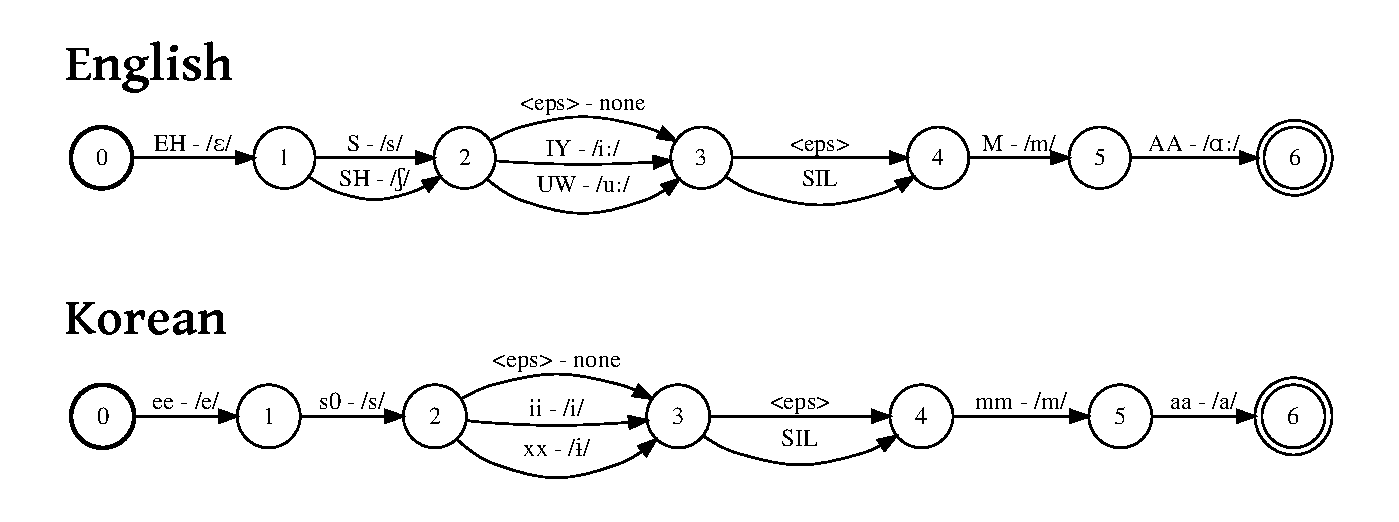
\includegraphics[width=0.9\linewidth]{chapter03/k-epenth_G.pdf}
    \caption{\textit{Constrained language model used to decode stimuli with the English (top) and Korean (bottom) acoustic models. The models here were used to decode items \textipa{/es([i|1])ma/}, as well as \textipa{/eS([i|1])ma/}. This is because there is only one \textipa{/s/} phoneme in Korean. As a consequence, we neutralised \textipa{/s/} and \textipa{/S/} for the English model to use either phoneme in a similar way. However this rarely happened in practice. Nodes in the graph represent states, edges represent transitions between states (here: phonemes). WSJ/KCSS labels are shown on edges, along with their IPA transcriptions. The LMs are null, as they only constrain the possible decoding outputs without assigning higher or lower probabilities to certain edges. The optimal decoding path is therefore only dependent on the acoustic scores.}}
    \label{fig:k-epenth_G}
  \end{figure}
  
\paragraph{Identification task simulation}
After decoding the stimuli with the ASR models, we extracted from the resulting lattices each possible transcription of each item, and the corresponding acoustic and language model scores. %An example of how the ASR system decodes the experimental stimuli can be seen in Figure \ref{fig:k-epenth_align}.
From the (scaled) acoustic and language model scores we derived the item posteriorgrams, which indicate how probable a given transcription was given the audio input. We used these probabilities as proxies of the probability that a listener might exploit when performing reverse inference during speech perception, and therefore, the probabilities used when responding in an identification task. 

As such, for each item, we obtained a three-dimensional vector $ident_{model} = [p_{none}, p_{i}, {\color{red}p_{\textipa{1}}}]$, containing a discrete probability distribution, with a probability mass function linking the identification task options \{`none', `\textipa{i}', `\textipa{1}'\}, to their respective probabilities (i.e., posteriorgrams).
We can define the human equivalent $ident_{human} = [p_{none}, p_{i}, {\color{red}p_{\textipa{1}}}]$, which contains the percentage of responses for each item, after aggregating all participant responses.

\subsubsection{Results}

\paragraph{Identification accuracy}
\begin{figure}[htb!]
  \centering
  \begin{overpic}[page=6, width=0.6\linewidth]{chapter03/k-epenth_figs}\end{overpic} \\
  \vspace{0.25cm}
  \begin{overpic}[page=5, width=0.6\linewidth]{chapter03/k-epenth_figs}\end{overpic}
  \caption{\textit{Identification accuracy on items with a full medial vowel, for human listeners (top, data from \cite{durvasula2015}) and the respective simulations (bottom). Results are shown for a model trained on American English (left) and a model trained on Korean (right). Points with error bars show the mean and standard deviation, respectively. The box and whiskers plots display the distribution of the proportions across items (median, quartiles, extrema and outliers).}}
  \label{fig:k-epenth_acc}
\end{figure}

Figure \ref{fig:k-epenth_acc} shows human and model accuracy when identifying medial full vowels, such as \textipa{[1]} in \textipa{/et\super h1ma/}. While English listeners showed an almost perfect performance (mean accuracy: \textipa{[i]}: $98\%$; \textipa{[1]}: $96\%$), the English model had difficulty identifying vowels, especially after palatal consonants (mean accuracy: \textipa{[i]}: $71\%$; \textipa{[1]}: $85\%$). This may be due to an acoustic mismatch between the nonnative vowels in the stimuli and the native vowels in the training corpus.

Contrary to their English-speaking counterparts, Korean listeners showed more difficulty identifying \textipa{[1]} ($61\%$ accuracy) while achieving good performance for \textipa{[i]} ($93\%$). Numerically, we found a similar pattern in model results (mean accuracy: \textipa{[i]}: $89\%$; \textipa{[1]}: $81\%$). However, unlike Korean listeners, the Korean model did not consistently perform better in \textipa{[i]}-trials than in \textipa{[1]}-trials.

\paragraph{Proportion of epenthesis}
\begin{figure}[htb!]
  \centering
  \begin{overpic}[page=8, width=0.6\linewidth]{chapter03/k-epenth_figs}\end{overpic} \\
  \vspace{0.25cm}
  \begin{overpic}[page=7, width=0.6\linewidth]{chapter03/k-epenth_figs}\end{overpic}
  \caption{\textit{Identification patterns on items with consonantal clusters, for human listeners (top, data from \cite{durvasula2015}) and the respective simulations (bottom). Proportion of ``none'', ``i'', and ``u''/``\textipa{1}'' responses given by the American English (left) and Korean (right) ASR systems. Points with error bars show the mean and standard deviation, respectively. The box and whiskers plots display the distribution of the proportions across items (median, quartiles, extrema and outliers).}}
  \label{fig:k-epenth_ep}
\end{figure}

Human and model response patterns for items with consonant clusters are given in Figure \ref{fig:k-epenth_ep}.
Concerning the control English human and model responses, as expected, the predominant case is not experiencing epenthesis. Respectively, English listeners experienced epenthesis in only $1\%$ of the trials, while the English model's average posteriorgram for epenthesis was $15\%$. The model's data was noisier than for humans, but the performances for both human and model in English surpassed the Korean equivalents.

Indeed, Korean listeners experienced epenthesis in $78\%$ of the trials, and the Korean model's posteriorgrams for epenthesis averaged to the equivalent of $66\%$ of the trials. Mirroring the higher rates of epenthesis for the English model, the Korean model outputs lower rates of epenthesis than Korean listeners.

Overall, we saw that the models were able to show the crosslinguistic difference in rates of epenthesis, with low rates for English and high rates for Korean.

\paragraph{Effect of palatalisation on \textipa{/i/}-epenthesis}
\begin{figure}[htb!]
  \centering
  \begin{overpic}[page=9, width=0.6\linewidth]{chapter03/k-epenth_figs}\end{overpic}
  \caption{\textit{Proportion of \textipa{/i/}-epenthesis on trials with epenthesis in cluster items, separating according to whether $C_{1}$ is a palatal or alveolar consonant. The box and whiskers plots display the distribution of the proportions across items (median, quartiles, extrema and outliers).}}
  \label{fig:k-epenth_KR_palatal}
\end{figure}

Focusing on epenthetic vowel quality, \cite{durvasula2015} found that Korean listeners mostly epenthesized \textipa{[i]} after palatal consonants, while they epenthesized the ``default'' vowel \textipa{[1]} after alveolar consonants. This can be seen for Korean listeners in Figure \ref{fig:k-epenth_ep}, but a similar effect is not visible for the Korean model, for which the rates of \textipa{/i/}- and \textipa{/1/}-epenthesis are at similar values around $25\% - 50\%$. Figure \ref{fig:k-epenth_KR_palatal} shows the proportion of trials with epenthesis for which the epenthetic vowel quality was \textipa{/i/}. Indeed, the difference between palatal ($65\%$) and alveolar ($55\%$) consonants observed in the Korean model is negligible compared to that observed in human responses (over $30\%$ difference).  

\subsubsection{Summary}
In this experiment, we investigated if ASR systems with a null language model could reproduce psycholinguistic effects attributed to native phonotactics. More precisely, we based ourselves on a study on the perception of consonant clusters by Korean listeners, where their performance was compared to that of American English listeners.

The first question related to when listeners experience vowel epenthesis when listening to nonnative speech. 
The English group served as a control group; the authors expected low rates of epenthesis, as English phonotactics are less restrictive than Korean phonotactics. Indeed, this was the case, with Korean speakers experiencing epenthesis in most trials, unlike English speakers. Thought not as clear cut as for humans, we found a similar effect when comparing cluster decoding by Korean and American English ASR systems.

Concerning trials where there was a full medial vowel between the consonants, the models diverged from human behaviour; in general, the identification accuracy was lower than for humans (especially the English one).

A second question referred to phonological influences on epenthetic vowel quality.
The authors observed higher rates of \textipa{/i/}-epenthesis in palatal allophones of alveolar consonants, in detriment of the default vowel \textipa{/1/}. This prompted them to hypothesize that phonological alternations were influencing epenthetic vowelselection during perception. We examined this hypothesis by investigating if our models, which lack explicit abstract phonological rules or contraints, could reflect this palatal effect. The hypothesis being that palatal consonants might contain acoustic cues more similar to the front vowel \textipa{/i/} than to \textipa{/1/}. However, we did not find evidences of the effect in the output of our models. It would be interesting to see if the effect might come from phoneme co-occurrences as, for instance, the diphone \textipa{[c\super hi]} is more frequent than \textipa{[c\super h1]} (Figure \ref{fig:k-epenth_kspan}). This might explain, in part, higher rates of \textipa{/i/}- than \textipa{/1/}-epenthesis in /\textipa{c\super h}$C$/ clusters. However, we remain skeptical, following the discussion about the low predictive power of \textipa{n}-gram-based phonotactic models in the previous section. 

\begin{figure}[htb!]
  \centering
  \begin{overpic}[page=3, width=\linewidth]{chapter03/k-epenth_figs_KSPAN}\end{overpic}
  \caption{\textit{Diphone frequency of \textipa{[c\super hi]} and \textipa{[c\super h1]}, relative to all diphones in Korean. Frequencies are computed from the frequencies of word types (top) and word tokens (bottom), as documented in K-SPAN \cite{holliday2017}.}}
  \label{fig:k-epenth_kspan}
\end{figure}

%%%%%%%%%%%%
% art2ac-per %
%%%%%%%%%%%%

\newpage
\subsection{{\color{red}Experiment 2: Position dependencies and syllabic structure}}
\small{\textit{{\color{red}ADD ACKNOWLEDGEMENTS EWAN, AMELIA KIMBALL, ANTOINE HEDIER, CLARA DELACOURT, PAUL ANDREY, EMMANUEL, MILICA (thank for recordings)}}}

In this experiment, we introduced basic allophony to the acoustic models of our ASR system, and evaluated whether this modification resulted in a better approximation of human responses in a task probing epenthesis. More specifically, we trained two different acoustic models which differed in whether phones were word-position-dependent (i.e., different HMM-GMMs depending on the position within the word) or not. We trained the models using the WSJ American English corpus, in order to model the perception of phonotactically illegal Serbian clusters by American English listeners. The clusters were either word-initial or word-medial. We expected American English listeners to experience epenthesis less frequently with word-medial clusters, as these clusters were legal across syllable boundaries. We examined whether this was the case and, if so, whether word-position-dependent models better approximated participants' rates of epenthesis than non-word-position-dependent ones.         

\subsubsection{Methods}
\paragraph{Stimuli}
We recorded a female native speaker of Serbian from Kruševac in a sound proof room reading a list of {\color{red}$X$} items containing a $C_{1}C_{2}$ cluster either in word-initial position ($C_{1}C_{2}V_{1}C_{3}V_{1}$, e.g., \textipa{/znapa/}) or word-medial position ($V_{1}C_{1}C_{2}V_{1}$, e.g., \textipa{/azna/}). $V_{1}$ and $C_{3}$ were always set to \textipa{/a/} and \textipa{/p/}, respectively. 
We also recorded the ``epenthesized'' equivalents of said stimuli, namely $C_{1}V_{ep}C_{2}V_{1}C_{3}V_{1}$ (\textipa{/z@napa/}) and $V_{1}C_{1}V_{ep}C_{2}V_{1}$ (\textipa{/az@na/}) with $V_{ep}$ set as \textipa{[@]}.
For all stimuli stress fell on the first $V_{1}$.
{\color{red}The list of stimuli is given in Table X.}

\paragraph{Behavioural experiment}
{\color{red}XX} monolingual native listeners of American English were recruited through the online platform Amazon Mechanical Turk. An additional {\color{red}XX participants were also tested, but they were excluded from the analyses if they met at least one of the following conditions: did not finish all trials, extensive exposure to languages other than English, auditory problems, dyslexia, unable to use headphones or earbuds during the experiment}. This information was retrieved from pre-test and post-test questionnaires.

After audio setup\footnote{Participants were given the opportunity to setup the audio to comfortable hearing levels.} and {\color{red}$XX$} training trials, in each experimental trial participants heard an item (e.g., \textipa{/azna/}). Since the grapheme-to-phoneme mapping is not as transparent in English as it is in Japanese or Korean, and because the position of the cluster in the item was not fixed, the task was slightly altered compared to other experiments described in previous sections. Participants were not asked if they had heard a vowel between the consonants; instead, they were given a 2-alternative forced choice task with orthographic transcriptions: if the auditory stimulus was \textipa{/azna/}, participants would be given the options \textit{``azna''} and  \textit{``azana''}. Since online participants are not as immersed in the experiment as participants tested in a laboratory setting, the experiment was self-paced and participants were able to listen to the stimuli as many times as necessary.

Each participant completed {\color{red}$XX$} trials. For each item, participants heard either the cluster version (e.g., \textipa{/azna/}) or the ``epenthesized'' version (e.g., \textipa{/az@na/}). Presentation of trials was counterbalanced between participants.   


\paragraph{ASR systems}
%\paragraph{Acoustic models}
We simulated perception of nonnative nonwords by English listeners using acoustic models trained on American English data (WSJ corpus). As in previous experiments, we used HMM-GMM monophone models with $15000$ Gaussians. However, we tested two types of acoustic models:

\begin{enumerate}
\item WPD-False (non-word-position-dependent) acoustic models: These are the type of models that have been used in all previous sections. For these models, all acoustic realisations of a phoneme are grouped together in a unique HMM. Therefore, for instance, in these models there is only one HMM corresponding to the phoneme \textipa{/p/}.
  \item WPD-True (word-position-dependent) acoustic models: In these models, different HMM-GMMs are built for phones, according to their position in a word (initial, medial, final, isolate). Therefore, there will be four separate HMM-GMMs for the phoneme \textipa{/p/}.  
\end{enumerate}

WPD-False and WPD-True acoustic models are allocated the same number of Gaussians, even though the latter have more phones (up to four times more than WPD-False models). This means that it is almost certain that the average number of Gaussians per phone HMM-GMM is lower in WPD-True than in WPD-False acoustic models. Also, since now acoustic realisations are separated according to their position in a word, we expect Gaussians to be distributed differently amongst HMM-GMMs.

{\color{red}[TODO] Show WER and PER differences on WSJ for wpdT vs wpdF}

%\paragraph{Modelling: Language models}
Concerning the language model used for decoding stimuli, item-specific language models were constructed, as shown in Figure \ref{fig:wpd_G}. For instance, when decoding an item /$C_{1}C_{2}$\textipa{apa}/, the perception model was only given the possibility to transcribe it as /$C_{1}(V_{ep})C_{2}$\textipa{apa}/, where phones between parentheses are optional and $V_{ep} = $ \textipa{[@]}. %And similarly for $V_{1}C_{1}(V_{ep})C_{2}V_{1}$ items.
While all non-medial vowels were intended to be \textipa{/a/} phonologically, we allowed the model to transcribe them as any phoneme associated with the grapheme $\langle a \rangle$. This allowed us to account for phonetic reduction in our stimuli, but also to account for the possibility that these alternative transcriptions might also be considered by English-speaking participants in the psycholinguistic experiment, due to item transcriptions being presented orthographically on-screen.

We use a null language model as shown in Figure \ref{fig:wpd_G}, meaning that the decoding process is entirely dependent on the acoustic model, without using information on phonotactics. Note that since we did not constrain the WPD-T model to only transcribe WPD allophones in their respective positions (e.g., allowing only the word-initial allophone of \textipa{/z/} between states $1$ and $2$ of the LM for \textipa{/znapa/}, but not the isolated \textipa{/z/} allophone), we are only comparing the two AMs based on their catalogues of phones, not on word-position matching of said phones.   

\begin{figure*}[htb]
\centering
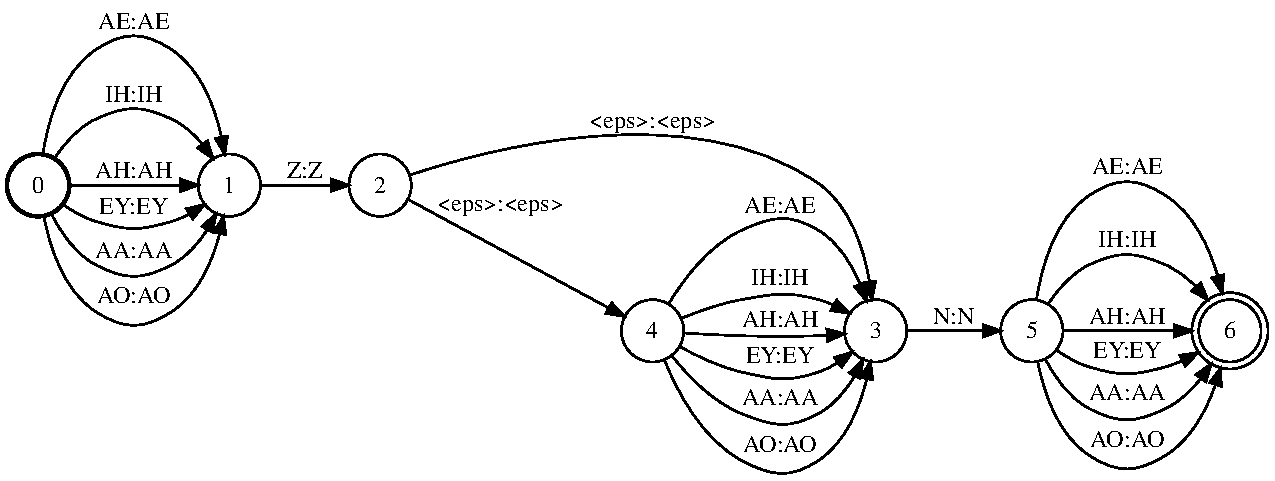
\includegraphics[width=0.8\linewidth]{chapter03/wpd-G_azna.pdf}
\vspace{0.5cm}
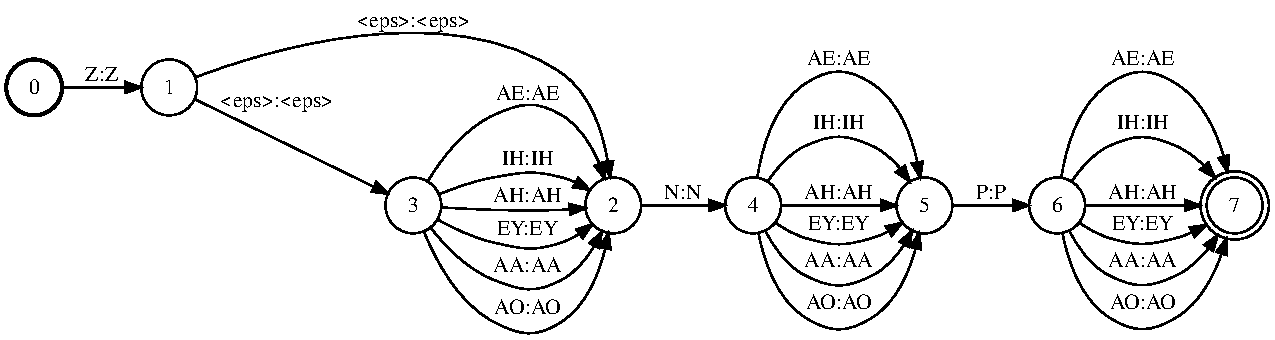
\includegraphics[width=0.8\linewidth]{chapter03/wpd-G_znapa.pdf}
\caption{Constrained language model used for stimulus decoding (here: LMs for \textipa{/azna/} (top) and \textipa{/znapa/} (bottom) trials). Nodes in the graph represent states, edges represent transitions between states (here: phonemes, transcribed in WSJ notation). Models were given the choice to transcribe the phoneme \textipa{/a/} with any of the phonemes linked to the grapheme $\langle a \rangle$, as English listeners might have also done so during the task. The LMs are null, as they only constrain the possible decoding outputs without assigning higher or lower probabilities to certain edges. The optimal decoding path is therefore only dependent on the acoustic scores.}
\label{fig:wpd_G}
\end{figure*}

\paragraph{Identification task simulation}
After decoding the stimuli, we obtained for each possible transcription of each item the corresponding acoustic and language model scores. From these we derived the item posteriorgrams; we collapsed together reponses with and without epenthesis, respectively. As such, posteriorgrams indicated the probability of epenthesizing \textipa{[@]} given the acoustic input. We used these probabilities as proxies of the probability that a listener might exploit when performing reverse inference during speech perception, and therefore, the probabilities used when responding in an identification task. In other words, for each item, we obtained a percentage of vowel epenthesis\footnote{For simplicity reasons, the term ``epenthesis'' will sometimes be used for items with full medial vowels (e.g., \textipa{/az@na/}), even though this is technically incorrect.}.

\subsubsection{Results}
  
\paragraph{Qualitative analysis}

\begin{figure}[htb!]
  \centering
    \includegraphics[page=3, width=0.45\linewidth]{chapter03/art2ac_model_pgrams.pdf}% \\
    \hspace{0.5cm}
    \includegraphics[page=4, width=0.45\linewidth]{chapter03/art2ac_model_pgrams.pdf}
    \caption{\textit{Experimental results for American English listeners.
      Left: Proportion of epenthesis, collapsed across participants. Clusters are ordered according to rates of epenthesis in word-initial clusters. 
      Right: Identification accuracy, according to the position of the cluster within the word and presence or absence of a vowel between the consonants. The box and whiskers plots display the distribution of the proportions across items (median, quartiles, extrema and outliers).}}
    \label{fig:wpd-hum}
  \end{figure}

The left panel of Figure \ref{fig:wpd-hum} shows the average percentage of epenthesis given by human participants for each item. Clusters are ordered according to the ranking of word-initial $C_{1}C_{2}$ clusters. We see that human participants were generally good at detecting \textipa{[@]} between two consonants, but their performance was not perfect, in particular when the target phonemes were word-initial. Concerning $C_{1}C_{2}$ clusters, there is a large range of rates of epenthesis for word-initial items, going from almost no epenthesis for \textipa{/tk/} to almost $75\%$ epenthesis for \textipa{/mr/}. For word-medial clusters we do not see the same variation in epenthesis, as most clusters ellicited epenthesis less that $25\%$ of the times. However, we do see that clusters are ordered relatively similarly to word-initial counterparts (e.g., the lowest and highest rates of epenthesis are for \textipa{/tk/} and \textipa{/mr/}, respectively). Note that, while most of the clusters are phonotactically illegal as syllable onsets in English, clusters that ellicited less epenthesis are not necessarily only the few clusters that are indeed legal (range from \textipa{/br/}: $6\%$ to \textipa{/gl/}: $31\%$). Indeed, as can be seen in Figure \ref{fig:wpd-legal}, most syllable-initial illegal clusters ellicit rates of epenthesis similar to those ellicited by legal clusters. 

\begin{figure}[htb!]
  \centering
    \includegraphics[page=8, width=0.4\linewidth]{chapter03/art2ac_model_pgrams.pdf}    \caption{\textit{Distribution of rates of epenthesis for human responses on word-initial clusters, according to phonotactic legality in onset position. Densities show the distributions normalised within each category of phonotactic legality.}}
    \label{fig:wpd-legal}
  \end{figure}

  Next we examined if, as predicted based on phonology, English listeners experienced lesser amounts of misperceptions when the clusters can be parsed as a sequence of a coda and an onset (word-medial cluster), instead of a complex onset (word-initial cluster). 
Statistical analyses were performed with the R statistical software \cite{R-base}, using Markov chain Monte Carlo linear models \cite{R-MCMCglmm, R-coda}. These Bayesian models sample coefficients from the posterior probability distribution conditioned on the data and given priors. We used priors that are standard for linear models. Model convergence was assessed by visual inspection of trace plots and the Gelman–Rubin convergence diagnostic \cite{gelman1992}, using eight chains with different initialisations. Effects were considered statistically significant if the 95\% highest posterior density (HPD) interval estimated for the coefficient of interest did not include zero. We report both the posterior mode and the 95\% HPD interval.  

Our response variable was the continuous variable \textsc{\%Accuracy}.
We chose as fixed effect for our statistical models \textsc{Position} (categorical variable with 2 levels: medial \textit{vs.} initial, contrast coded with deviation coding) and \textsc{Vowel} (categorical variable with 2 levels: true \textit{vs.} false, contrast coded with deviation coding), as well as their interaction.

The right panel of Figure \ref{fig:wpd-hum} shows the percentage of accuracy for human participants. We found a significant main effect for \textsc{Position} (mode: $-0.11$, HPD: $[-0.15, -0.07]$), \textsc{Vowel} (mode: $-0.07$, HPD: $[-0.11, -0.03]$), as well as their interaction (mode: $-0.12$, HPD: $[-0.18, -0.02]$). English listeners were generally better at detecting a present vowel (i.e., no incorrect elision) than at correctly parsing clusters (i.e., no incorrect epenthesis). They experienced more misperceptions at trials where the cluster was word-initial, even more so for $C_{1}C_{2}$-items than for $C_{1}$\textipa{[@]}$C_{2}$-items. %\\

%%%%%%%  
\begin{figure}[htb!]
    \centering
    \includegraphics[page=5, width=0.45\linewidth]{chapter03/art2ac_model_pgrams.pdf}%\\
    \hspace{0.5cm}
    \includegraphics[page=6, width=0.45\linewidth]{chapter03/art2ac_model_pgrams.pdf}

    \caption{\textit{Simulation results for ASR models.
      Left: Epenthesis posteriorgrams. Clusters are ordered according to rates of epenthesis in word-initial clusters given by human participants. 
      Right: Identification accuracy, according to the position of the cluster within the word and presence or absence of a vowel between the consonants. The box and whiskers plots display the distribution of the proportions across items (median, quartiles, extrema and outliers).}}
    \label{fig:wpd-mod}
  \end{figure}

  Model responses can be seen in Figure \ref{fig:wpd-mod}. On the left panel, we can see that the models almost never elide full vowels (light gray datapoints). This results in almost perfect performance for these items, as seen in the right panel.
  On the other hand, there is large variability in the posteriorgrams for $C_{1}C_{2}$ clusters, even for word-medial items. This is also visible from the elongated black boxplots on the right panel. Recall that English listeners gave a large range of percentages for word-initial items only, while they experienced lower rates of epenthesis for word-medial clusters.
  Closer examination of epenthesis rates according to the ranking of the clusters in the left panel reveals that for word-initial clusters the models generally agree with humans as to which clusters ellicit more (e.g., \textipa{/gn/}, \textipa{/mr/}, \textipa{/dn/}) or less (e.g., \textipa{/zg/}, \textipa{/dl/}, \textipa{/kl/}) epenthesis.
  We did not analyse the model data as we did for human data, due to issues related to highly skewed distributions for full vowel items, and too much variability for cluster items (almost uniform distribution in the [0,1] interval). However, from looking at both panels from Figure \ref{fig:wpd-mod}, we can hypothesize that models also misperceived $C_{1}C_{2}$-items more often than $C_{1}$\textipa{[@]}$C_{2}$-items. Yet, it is difficult to find evidence for lessened misperception of clusters in word-medial position.  

\paragraph{Quantitative analysis}

\begin{figure}[htb!]
    \centering
    \includegraphics[page=7, width=0.7\linewidth]{chapter03/art2ac_model_pgrams.pdf}
    \caption{\textit{Models' epenthesis posteriorgrams as a function of the percentage of epenthesis given by humans for a given $C_{1}C_{2}$ cluster (black) or $C_{1}$\textipa{[@]}$C_{2}$ (light gray) item. Dashed lines indicate identity.}}
    \label{fig:wpd-corr}
  \end{figure}

  The relationship between human responses and model estimation can be visualized in Figure \ref{fig:wpd-corr}. In order to perform a global evaluation of the similarity between human responses and the responses given by the WDP-F and WPD-T models, respectively, we used leave-one-out cross-validation. This method consists of computing $\textsc{CV}$, the average prediction error on an item $i$ by a statistical model trained on all items except $i$. We used the following linear models (one per AM) as predictive models:

  \begin{equation}
    \textsc{\%epenth}_{human} = \textsc{\%epenth}_{model} \times \textsc{Position} \times \textsc{Vowel} + \epsilon
  \end{equation}

  In other words, we compared the predictive power of linear models using as predictor variables the model posteriorgrams ($\textsc{\%epenth}_{model}$), the cluster position (\textsc{position}; medial \textit{vs.} initial), the presence of a full vowel (\textsc{Vowel}; true \textit{vs.} false), their interactions, and residuals ($\epsilon$). The data to be predicted were human percentages of epenthesis per item ($\textsc{\%epenth}_{human}$).
  Contrary to expectations, we found the ASR system with the WPD-F acoustic model to have lower average prediction error ($\textsc{CV} = 0.014$) than the ASR system with the WPD-T acoustic model ($\textsc{CV} = 0.016$).
  
\subsubsection{Summary}
In this experiment we tested the perception of Serbian clusters (and their ``epenthesized'' counterparts) by native listeners of English. Most of these clusters were phonotactically illegal syllable-initially in English. We found that while English listeners were better at detecting the presence of a full vowel than detecting its absence, they still experienced elision on items with full vowels between the consonants of interest. However, the predominant category of mistakes is epenthesis. In particular, listeners experienced misperceptions more often when the clusters where word-initial than when they were word-medial. Additionally, amongst clusters that ellicited the least amount of epenthesis in word-initial position we find clusters that are phonotactically legal in this position, and other that are illegal.

We simulated the experiment above using ASR systems with two types of acoustic models: a WPD-F model, which groups all acoustics related to one phoneme within a unique phone, and a WPF-T model, which groups acoustics according to whether they originate from a word-initial, word-medial, word-final, or isolated phone.
We found that, globally, the WPD-F model better approximated human results. However, it appears that neither model is able to reproduce the lower accuracy for word-medial than for word-initial $C_{1}($\textipa{[@]}$)C_{2}$ items.
  
\subsection{General discussion}

%%%%%%%%%%%%%%%%%%%%%%%%%%%
% Chapter mini-discussion %
%%%%%%%%%%%%%%%%%%%%%%%%%%%
\newpage
\section{Conclusions}
%%% SUMMARY %%%

%%% SHORT DISCUSSION %%%

%%% LIMITATIONS %%%

% Need more faithful transcription to build LMs from!! (cf differences in epenthesis between BP and PP).
% Ideas:
%% --- Automatic iterative decoding from null model  
%% --- For specific phoneme sequences, find exemplars (e.g., for /hp/ check all /hVp/) and see if well transcribed. Adapt probabilities accordingly. PB: Need many exemplars + Time consuming. 

%%% Null model isn't really null in that transition probabilities in HMMs capture diphone probabilities already. Ideally, for a truly null model, need to modify topology and equalise all C->V TPs. But not identical to having just P(V|C). [CHECK THOMAS]

% Need better acoustic model. But we need not to integrate triphones.
% Ideas:
%% --- NN-based ASR systems (monophones)
%% --- End-to-end training

%%% k-epenth
%EN vs KR: Cross-linguistic effect or due to corpora???

%%% wpd
%low epenthesis rates for illegal clusters: due to adaptation (cf tl->kl in FR)? Deletion? Or genuinely acoustics > phonology?  

%%% How to account for results by:
% - Durvasula & Kahng (2016): Different rates of epenthesis for [km] and [gm], the latter being legal across IP boundaries. Increased voicing => increased epenthesis, even when splicing out consonantal release. 
% - Kabak & Idsardi (2007): Better AX performance for clusters with legal coda consonant, even if cluster was illegal.
% ==> Acoustic productions in certain clusters are more acceptable as allophones of syll/IP final legal Cs than the counterpart for non-legal Cs?
% Role of markedness (cf Berent 2007)? 
%%% - Sonority scale has acoustic basis (Yun's thesis)
%%% - Articulatory basis? More marked structures impose more constraints on the resulting acoustics, making them less likely to ressemble exemplars of the same phoneme from less marked structure?
%%% Test through splicing experiments? (e.g. lbif with another l). But need to be careful with acoustics...


%%% Conclusions